\documentclass[a4paper, 12pt, twoside, english]{article} 


% Incorporate the preamble
\usepackage{preamble}



%=============================================================================================================================================================================





\begin{document}


\def\biblio{} % resets the biblio command, if not here a new reference list will be produced after every chapter










\begin{titlepage}
	

	\begin{center}
	
	\scshape % Use small caps for all text on the title page
	
\includegraphics[width=1 \linewidth]{IFME/Graphs/uniol_4c.pdf}
	\vspace*{\baselineskip} % White space at the top of the page
	\vspace{-1.5cm}
	%------------------------------------------------
	%	Title
	%------------------------------------------------
	
	\rule{\textwidth}{1.6pt}\vspace*{-\baselineskip}\vspace*{2pt} % Thick horizontal rule
	\rule{\textwidth}{0.4pt} % Thin horizontal rule
	\vspace{-0.9cm}
	\vspace{0.35\baselineskip} % Whitespace above the title
	
	{\rmfamily\scshape\LARGE  \textbf{Topic Title\\}} % Title
	
	\vspace{0.35\baselineskip} % Whitespace below the title
	
	\rule{\textwidth}{0.4pt}\vspace*{-\baselineskip}\vspace{3.2pt} % Thin horizontal rule
	\rule{\textwidth}{1.6pt} % Thick horizontal rule
	
	\vspace{0.1\baselineskip} % Whitespace after the title block
	
	%------------------------------------------------
	%	Subtitle
	%------------------------------------------------

    Own Subtitle% Subtitle or further description
	
	\vspace*{1.5\baselineskip} % Whitespace under the subtitle
    
    \end{center}
    
	%------------------------------------------------
	%	Editor(s)
	%------------------------------------------------

            




\begin{center}
    \begin{minipage}[t]{0.45\textwidth}
        \begin{flushleft}
            \textbf{\underline{Author}:} \\
            \textit{Jannes Ehrhardt (5257507)$^{\text{ \textbf{JE}}}$} \\
            \textit{\href{mailto:jannes.ehrhardt@uni-oldenburg.de}{jannes.ehrhardt@uol.de}}
        \end{flushleft}
    \end{minipage}%
    \hspace{0.1\textwidth}%
    \begin{minipage}[t]{0.45\textwidth}
        \begin{flushright}
            \textbf{\underline{Supervising Examiner}:} \\
            \textit{Prof. Dr. Hans-Michael Trautwein} \\
            \textit{\href{mailto:hans.michael.trautwein@uni-oldenburg.de}{hans.michael.trautwein@uol.de}} \\
        \end{flushright}
    \end{minipage}
    \vspace*{1\baselineskip}
\end{center}








	\begin{center}













    
	\rmfamily\scshape   
	   
	   
	   
	\textbf{\Large{Applied Economics}} \\ 
    (wir873) \\
    \vspace{.4cm}
	\textbf{Paper} \\
    \vspace{.4cm}
	Institute for Economics \\
	
	   
	\vspace*{2.0\baselineskip} % vor Änderung das Uni-Logo war das hier eine 3 
	
	%------------------------------------------------
	%	Publisher
	% 
\includegraphics[width=1 \linewidth]{Graphs/uniol_4c.pdf}
	%------------------------------------------------
	
	%\plogo % Publisher logo
	
	% \vspace{.7\baselineskip} % Whitespace under the publisher logo

 \normalfont
    Oldenburg, \today
	
	
		\pagenumbering{Roman}
%\addcontentsline{toc}{section}{Titlepage}   %einfügen ins Inhaltsverzeichnis
	
	\end{center}




\end{titlepage}









%\newpage
%{\setstretch{1.25} 
%\listoffigures}

 
%\newpage
%{\setstretch{1.25} 
%\listoftables}

\newpage
\restoregeometry % restores the margins after frontpage
%\nocite{*} % uncomment if you want all sources to be printed in the reference list, including the ones which are not cited in the text 

\pagenumbering{gobble} % suppress page numbering
\thispagestyle{plain} % suppress header
%\clearpage\mbox{}\clearpage % add blank page

\pagenumbering{Roman} % starting roman page numbering
\newpage
%\section*{Acknowledgements}
%    \subfile{Vorwort/Acknowledgements}
\setcounter{page}{2}   % start der seitenzahl im Abstract 
%\newpage
\section*{Abstract}
\addcontentsline{toc}{section}{Abstract}
    \subfile{Foreword/Abstract}


\newpage


\renewcommand{\contentsname}{\Large{Table of Contents}}
\section*{}
% \vspace{-1,5cm}
\addcontentsline{toc}{section}{Table of Contents}
{\setstretch{1.25} % line spacing for the list
{\hypersetup{linkcolor=Black} % Make toc black even if general linkcolor is different
\tableofcontents
}
}





\newpage




\renewcommand{\listfigurename}{\Large{List of Figures}}
\section*{}
% \vspace{-1,5cm}
\addcontentsline{toc}{section}{List of Figures}
{\setstretch{1.25}
{\hypersetup{linkcolor=Black}
\listoffigures
}
}




\newpage




\renewcommand{\listtablename}{\Large{List of Tables}}
\section*{}
% \vspace{-1,5cm}
\addcontentsline{toc}{section}{List of Tables}
{\setstretch{1.25}
{\hypersetup{linkcolor=Black}
\listoftables
}
}
\newpage



\addtocontents{toc}{\protect\setcounter{tocdepth}{4}} % sets depth of toc to 4, 1.1.1.1
\pagenumbering{arabic} % Starting arabic page numbering
\setcounter{page}{1} % sets pagecounter to 1





%\newpage
%\renewcommand\refname{References} % name for the reference list
%{\setstretch{1.0} % linespacing for the references
%\addcontentsline{toc}{section}{References} % to change the name of the references in the TOC
%}

%\newpage
%\renewcommand{\appendixpagename}{Appendix} % Heading of appendix
%\renewcommand{\appendixtocname}{Appendix} % name of appendix in TOC
%\appendixpage 
%\addappheadtotoc















\section[Introduction]{Introduction$^{\text{ AA, JE, MK}}$} 
\label{sec:Introduction}

That international trade and specialization can potentially generate welfare gains has long been recognized by economic literature. Especially in developed nations, the service sector has become increasingly important. This development holds true for cross-border services. Since the 1990s trade in services had the highest growth rates compared to other dimensions of international trade (\cite{Breinlich_and}). As global value chains become more integrated with the emergence of cross-border services that can be used as input factors in production (\cite{understanding_2023}), keeping track of the patterns of trade is an ongoing task for empirical research. 

A robust finding is that the gravity model introduced by \textcite{tinbergen1962shaping} can be utilized as an econometric tool to analyze the determinants of trade and identify anomalies that have important policy implications (\cite[p. 41]{krugman2019}). Moreover, the model has been progressively enhanced by empirical refinements, such as the extension by \textcite{Anderson2003} to transfer the originally bilateral model into a multilateral one. \enquote{Hundreds of papers have used the gravity equation to study the effects of geography, demographics, RTAs, tariffs, exports subsidies, embargoes, trade sanctions, the World Trade Organization member- ship, currency unions, foreign aid, immigration, foreign direct investment, cultural ties, trust, reputation, mega sporting events (Olympic Games and World Cup), melting ice caps, etc. on international trade.} (\cite[p. 17]{yotov2016advanced}). This quote summarize the wide applicability of the model quit well.

The original gravity model was however designed for countries that engage in trade of physical merchandise products (from here on we simply call that \textit{trade in goods}), not for cross-border services. Recent literature continuous to adjust the gravity framework, making use of newly developed methods, to also apply the intuitive idea of gravity to other subjects of trade. In this seminar paper, we highlight the differences of gravity based approaches in respect to traded goods and traded services. We aim at providing a comprehensive and useful overview as an introduction to this large literature branch.

Trade barriers and related costs are of particular interest in the empirical literature and in theoretical models. The findings suggest that these play a huge role in determining bilateral trade flows with regards to the establishment of relationships, but also to the volume traded. Therefore, we believe that trade barriers and costs have a high policy relevance. Furthermore, we find that the assessment of trade barriers and costs tends to be a more demanding task for empirical analysis of trade in services, than for trade in goods. This can mainly be explained by the intangible nature of services, the high level of firm heterogeneity in service sectors and the complex interdependencies in global value chains.


The rest of this paper is organized as follows. Section \ref{sec:Gravity_Framework} presents the gravity model by discussing its theoretical linkages to international trade theory and reviewing the empirical tools and challenges that readers have to be aware of when dealing with gravity literature. We then dedicate section \ref{sec:Determinants_of_Trade} to the exploration barriers and costs of trade. Section \ref{sec:Empirical_evidence} discusses implications and results of selected papers for both goods and services applications and finally, section \ref{sec:conclusion} concludes.
















































































\section[The Gravity Framework in international Trade]{The Gravity Framework in international Trade$^{\text{ AA, JE}}$}
\label{sec:Gravity_Framework}

The gravity model of trade has its roots in Newtonian physics, where the force of gravity between two objects is directly proportional to their masses and inversely proportional to the square of the distance between them. Similarly, the gravity equation in international trade posits that the volume of trade between two countries is directly proportional to their economic size, usually measured by GDP, and inversely proportional to the distance between them. \textcite{tinbergen1962shaping} is often cited as the first to apply this concept to international trade, proposing that larger economies trade more with each other and that trade diminishes with increasing distance.

\textcite{Anderson2003} introduced significant refinements to the gravity model by addressing the issue of \textit{multilateral resistance}. They argued that trade flows between two countries depend not only on their bilateral distance but also on their relative distances to all other trading partners. This adjustment accounts for the fact that a country’s trade is influenced by its position in the global trade network.

Due to the high amount of textbooks and scientific papers that incorporated the gravity framework over the last decades, formal notations differ substantially. In this section, we present the linkages of the gravity framework to international trade theory and discuss the main empirical estimation strategies to provide the reader with a basic understanding of challenges when it comes to combining theory with data. Therefore, we utilize the notation style of \textcite[p. 17]{yotov2016advanced}, who provide an advanced guide for researchers who aim to construct a gravity analysis. To capture both the original idea of \textcite{tinbergen1962shaping} and the extension of \textcite{Anderson2003}, they denote the \textit{structural gravity model} as shown in equation \ref{eq:Structural_Model_NF}: \begin{equation}
    \label{eq:Structural_Model_NF}
    X_{ij} = \Tilde{G} \frac{Y_i E_j }{T_{ij}^{\Theta}}
\end{equation} In this notation $X_{ij}$ represents exports from country i and j, $\Tilde{G}$ is the inverse of the total world production ($\Tilde{G} \equiv 1/Y$), $Y_i$ is country $i$'s domestic production, $E_i$ is country $j$'s aggregate expenditure and $T_{ij}^{\Theta}$ are the total trade costs between countries $i$ and $j$. Finally, $T_{ij}^{\Theta} \equiv \left( t_{ij}/(\Pi_i P_j) \right)^{\sigma - 1}$ is a term that includes all costs of trade, where $t_{ij}$\footnote{Finding fitting proxies for $t_{ij}$ is an ongoing challenge in the empirical literature and will be discussed in depth in section \ref{sec:Determinants_of_Trade}.} are bilateral trade costs between economies, $\Pi_i$ is a structural term to capture the idea of multilateral resistance by \textcite{Anderson2003} and can be interpreted as market access abilities of an exporting country $i$ (\textit{outward} multilateral resistance), while $P_j$ captures an importing country's market access ability as \textit{inward} multilateral resistance (\cite[p. 16]{yotov2016advanced}).\footnote{\textcite[pp. 13-17]{yotov2016advanced} also provide a formal demand side derivation of the structural gravity model, while a supply side derivation is shown in their appendix.} Considering a model with $t$ periods, to obtain an easily estimable structural gravity equation, expression \ref{eq:Structural_Model_NF} can be log-linearized. \begin{equation}
    \label{eq:Structural_Model_LIN}
    \ln{X_{ij,t}} = \ln{E_{j,t}} + \ln{Y_{i,t}} - \ln{Y_t} + (1-\sigma) \ln{t_{ij,t}} - (1-\sigma) \ln{P_{j,t}} - (1-\sigma) \ln{\Pi_{i,t}} + \epsilon_{ij,t}
\end{equation} Equation \ref{eq:Structural_Model_LIN} than represents a theory founded model that can be estimated using econometric methods. Note that the error term $\epsilon_{ij,t}$ is introduced to capture noise in the data (\cite[p. 17]{yotov2016advanced}). In what follows, a brief overview of how equations \ref{eq:Structural_Model_NF} and \ref{eq:Structural_Model_LIN} are linked to well developed international trade theories (section \ref{subsec:theoretic_foundations}) is given. Furthermore, challenges when it comes to estimating equation \ref{eq:Structural_Model_LIN} are reviewed (section \ref{subsec:estimation_tools}) in order to generate a basic understanding of the discipline. This enables the reader to better focus on the reasoning in following chapters.











\subsection[Theoretic Foundations]{Theoretic Foundations$^{\text{ AA}}$}
\label{subsec:theoretic_foundations}

Trade has always been acknowledged as a factor, in promoting unity and fostering peace among nations. The belief that interconnected markets lead to benefits and stability has historical roots, especially evident in the relationship between the U.S. And Europe, where trade has often played a role in maintaining peace and strengthening economic connections. This viewpoint holds relevance today given the increasing tensions and the volatile nature of the global economy. Therefore analyzing trade patterns and understanding what drives trade have become tasks for researchers seeking to shed light on how trade can contribute to stability and prosperity.

The gravity model stands out as a tool for studying trade dynamics. Similar to its namesake concept in physics this model suggests that the volume of trade between two countries is directly related to their sizes while being inversely proportional to the distance separating them. This model has demonstrated power in understanding trade patterns and has been widely utilized to identify irregularities and explore the factors influencing trade volumes. Renowned economist Paul Krugman emphasizes the significance of gravity analysis in uncovering these irregularities and examining socio linguistic and geographic factors that affect international trade .

Inspired by Newtons law of gravity the gravity model of trade has long been a principle, in economics.
This theory suggests that the amount of trade, between two countries is directly linked to their strength usually measured by GDP and inversely related to the distance separating them (\cite{tinbergen1962shaping}). While using gravity equations has shed light on the patterns and factors influencing goods trade the changing global economy requires an evaluation of their relevance to services trade.

Since the 1990s services trade has shown growth rates compared to aspects of international trade (Breinlich et al. as cited in WTO). Services have become a part of trade covering various activities like financial services, tourism, information technology and professional services. Unlike goods trade services involve features such as intangibility, diversity and the need for interactions between producers and consumers. This often blurs regulatory boundaries. These differences lead to questions; do gravity equations work well for goods and services trade? Are the factors influencing and hindering trade the same, in both sectors?

This article explores these questions by offering an examination of gravity equations concerning goods and services trade.
The gravity model is thoroughly explored in this study analyzing research findings and emphasizing the varying impacts of distance economic size and other variables, on the trade of goods versus services. \textcite{Anderson2003} refined the model to address resistance factors for understanding trade dynamics in both sectors. \textcite{Kimura2006} underscored the need to consider service characteristics when using gravity equations as traditional models may not fully capture service trade dynamics.

Moreover studies by \textcite{NBERw12516} and \textcite{EGGER2011263} have shown that while gravity equations can apply to both goods and services their sensitivity to factors like distance and economic integration differs significantly between the two. \textcite{Bergstrand_1985} highlighted the roots of the gravity equation suggesting that distinct factors drive goods, versus services trade.

This analysis aims to determine whether a unified model can effectively capture the complexities of both goods and services trade or if adjustments are needed to accommodate the nature of services.
This study not enhances our comprehension of trade but also offers valuable perspectives for decision makers seeking to promote economic growth by easing trade restrictions.



% 6.Krugman, P. (2019). International Economics: Theory and Policy. [Page 41].


% 8.Yotov, Y. V., Piermartini, R., Monteiro, J. A., \& Larch, M. (2016). An Advanced Guide to Trade Policy Analysis: The Structural Gravity Model. [Page 17].



% Here comes the section about theoretic foundations:



\begin{figure}[htbp]
    \centering
    \caption[Gravity model's strong theoretical foundations]{Gravity model's strong theoretical foundations}
    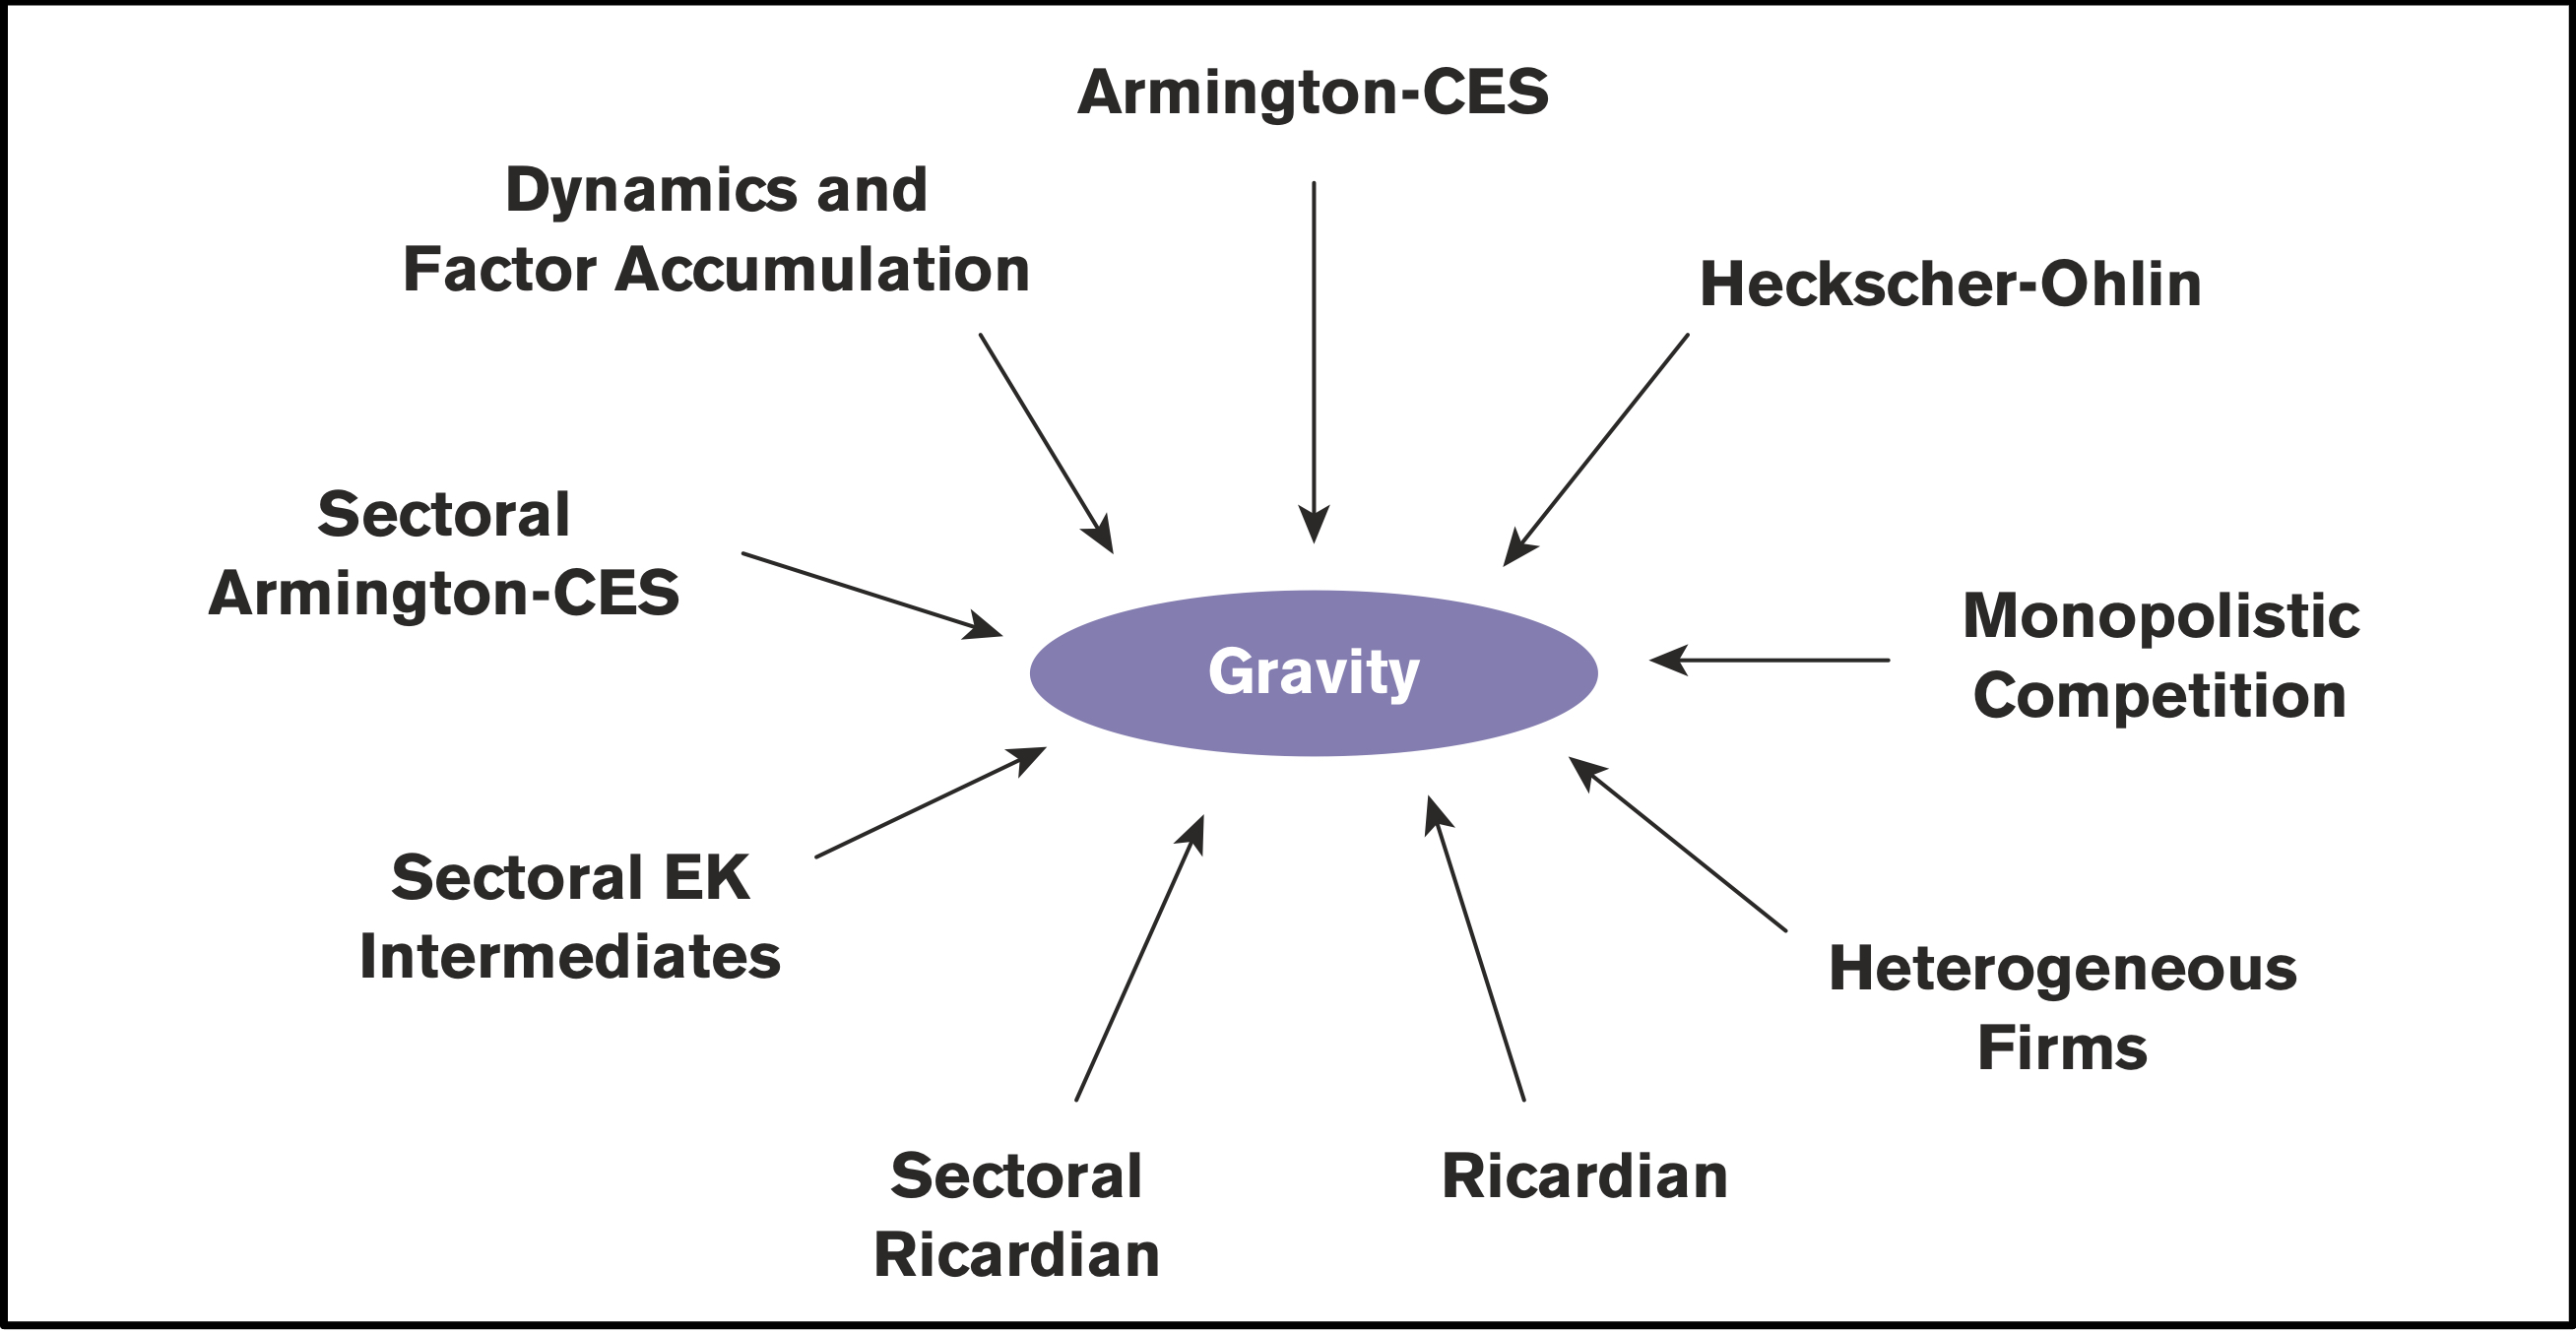
\includegraphics[width=1\textwidth]{IFME/Graphs/foundations.jpeg}
    \label{fig:theoretic_foundations}
    \small 
    Figure Source: \cite[p. 12]{yotov2016advanced}
\end{figure}

















\subsection[Estimation Tools and Challenges]{Estimation Tools and Challenges$^{\text{ JE}}$}
\label{subsec:estimation_tools}


Conveniently, gravity models can generate \textit{isomorphic} equations (\cite[p. 13]{yotov2016advanced}). This property means that the form of the trade gravity equation can be generalized or adapted to fit different contexts or additional relevant variables, maintaining its core structural properties. For instance, the simple gravity model can easily be prolonged by a vector of additional explanatory variables or elasticity parameters, like distance or cost elasticities. When it comes to equation \ref{eq:Structural_Model_LIN}, $t_{ij,t}$, $P_{j,t}$ and $\Pi_{i,t}$ are not directly observable in data. So there is a need for proxies that capture the implied trade costs and multilateral resistance terms sufficiently.   

Before \textcite{Anderson2003} highlighted the importance of multilateral resistance terms, the gravity trade model mainly had a bilateral setup. Identifying bilateral costs of trade therefore was (and still is) one of the main challenges in the estimation process. The standard procedure is to include covariates that can be observed through data and estimate the log-linearized equation \ref{eq:Structural_Model_LIN} using the ordinary least squares (OLS) estimator. \textcite[p. 21]{yotov2016advanced} list the following covariates as the most often incorporated ones: \begin{equation}
    \label{eq:bil_trade_costs_SGE}
    (1-\sigma) \ln{t_{ij,t}} = \beta_1 \ln{\underbrace{\text{DIST}_{ij}}_{\underset{\text{distance}}{\text{spatial}}}} + \beta_2 \underbrace{\text{CNTG}_{ij}}_{\underset{\text{dummy}}{\text{border}}} + \beta_3 \underbrace{\text{LANG}_{ij}}_{\underset{\text{dummy}}{\text{language}}} + \beta_4 \underbrace{\text{CLNY}_{ij}}_{\underset{\text{dummy}}{\text{colonial-ties}}} + \beta_5 \underbrace{\text{RTA}_{ij,t}}_{\underset{\text{dummy}}{\text{RTA}}} + \beta_6 \underbrace{\Tilde{\tau}_{ij,t}}_{\ln{(1+\text{tariff}_{ij,t})}}
\end{equation} Section \ref{sec:Determinants_of_Trade} will present further specifications of the bilateral trade costs. Note however that tariffs imposed by economy $j$ on exports from $i$ to $j$ at time $t$ enter the regression as $\ln{(1+\text{tariff}_{ij,t})}$ to avoid loosing observations in which there is no tariff.\footnote{There is no number $x$ such that $e^x=0$, so these observations would be dropped in an OLS regression.} This is important, since the trade elasticity of substitution ($\sigma$) is one of the main interests of researchers constructing gravity analysis and it can be approximated by the coefficient $\beta_6$ due to the fact that tariffs are direct price shifters of the traded goods and services (\cite[p. 21]{yotov2016advanced}).


The transition from only using a bilateral gravity setup to modeling a multilateral gravity equation also becomes a challenge when performing empirical estimation. \textcite{NBERw12516} introduce the term \textit{Gold Medal Mistake} as an expression for simply neglecting the multilateral resistance introduced by \textcite{Anderson2003}. $P_{j,t}$ and $\Pi_{i,t}$ from equation \ref{eq:Structural_Model_LIN} are not observed data but rather constructed in the derivation of the structural gravity model. However, not including any measures for these terms should bias the results, since their theoretical foundations of a multilateral system is still important for the gravity model. \textcite{Anderson2003} use a specific form of \textit{iterative custom nonlinear least squares programming}\footnote{The intuition is that the model is iteratively estimated over and over again with a flexible set of resistance terms until convergence, so the results do not change anymore (\cite[p. 18]{yotov2016advanced}).} to construct a set of multilateral resistances. A simpler approach would be to include so called \textit{remoteness indices} in the estimation. These indices are usually constructed in a way to capture bilateral distance and economic masses relative to world mass (expressed as GDP). \textcite{Kimura2006} for example use such a remoteness index to apply the gravity equation to trade in services.\footnote{Implications of \textcite{Kimura2006} will be discussed in later sections.} As indices constructed like that only proxy remoteness in a broad way and not fully resemble the theoretical idea of a multilateral trade system, more recent literature marks the their inclusion as insufficient to capture multilateral resistance. \textcite[p. 150]{cookbook} illustrate the issue like this: \begin{equation}
    \label{eq:REM1}
    \text{REM1}_n = \sum_i \left(\frac{\text{Dist}_{ni}}{Y_i}\right)
\end{equation} \begin{equation}
    \label{eq:REM2}
    \text{REM2}_n = \left(\sum_i \left(\frac{Y_i}{\text{Dist}_{ni}}\right)\right)^{-1}
\end{equation} In the remoteness index presented in equation \ref{eq:REM1}, very small countries are disproportionately accounted for, as $Y_i$ (GDP) is very small for them. The $\text{REM2}_n$ measure from equation \ref{eq:REM2} fixes this problem to some extend in the way that a very small $Y_i$ leads to lower effects when entering the regression as explanatory variable, as does a high $Dist_{ni}$. However, it is still not consistent with the underlying theory of remoteness factors in the way that the multilateral trade system is not represented properly (\cite[p. 151]{cookbook}). Additional alternatives to handle multilateral resistance terms would be (i) to drop them ($P_{j,t}$ and $\Pi_{i,t}$) out of equation \ref{eq:Structural_Model_LIN} by applying suitable ratios derived from equation \ref{eq:Structural_Model_NF}, (ii) to employ a dual version of the gravity model that uses techniques from spatial econometrics to include interdependence between trade flows of two economies and events happening in the rest of the world as suggested by \textcite{dualapproach}\footnote{This approach is well suited for cross-sectional data but is difficult to translate into a multi-period setup with panel data.}, or (iii) to use directional (exporter and importer) fixed effects for a cross-sectional data setup and directional time- and group-fixed effects for longitudinal data, respectively (\cite[p. 18-19]{yotov2016advanced}). One advantage of the fixed effects approach is that they will also control for other unobservables that vary over countries (policies etc.) or over time (outside shocks etc.).\footnote{\textcite[p. 152]{cookbook} even state that the inclusion of fixed effects can control for overstatements in data. They give the example of Belgium's port in Antwerp or Netherlands's port in Rotterdam to illustrate that a large amount of exports and imports flow through these stations. While the relevant trade data should only represent the commodities' origin country of production, used warehouses and reporting errors could lead to an overstatement of the port-countries exports (or imports). Such data discrepancies can also be absorbed by fixed effects (\cite[p. 152]{cookbook}). Note that this issue relates mainly to trade in goods, while for trade in services other problems arise (see section \ref{sec:Service_Models}).} Another pro-argument for the inclusion of fixed effects is that they can help to mitigate the estimation bias induced by potential (and likely) endogeneity of trade policies like RTAs. Such trade policies obviously are an important covariate when explaining trade patterns and determining the costs of trade. The decision to engage in contracts of lowering trade barriers is, however, also likely to be correlated to other explanatory variables (like distance or language barriers) and therefore brings up the issue of endogeneity (\cite[p. 21]{yotov2016advanced}). Finding and assessing relevant and exogenous instrumental variables is an ongoing struggle in the literature, especially for applications to international trade. That is why combining different econometric approaches with fixed effects and multiple robustness checks can be described as the go-to approach to address potential endogeneity of trade policies (\cite{trade_agreements_2024}, \cite[p. 21]{yotov2016advanced}).

While having the above mentioned advantages, the inclusion of fixed effects can also lead to problems in consistent estimations of gravity models, as they might absorb impacts that other covariates have on trade which are subject to the analysis. One prominent example are non-discriminatory trade policies\footnote{Non-discriminatory trade policies require that countries treat trading partners equally, offering the same terms to all under the \textit{most-favoured-nation} principle, and that imported goods receive the same treatment as domestic products, known as \textit{national treatment}. These principles aim to ensure fairness and prevent biases in international trade practices but can also be dominated by special forms of market integration like RTAs (\cite{wto_nondiscrimination}).} (\cite[p. 22]{yotov2016advanced}). The intuition is that if such policies are in place, the analyst is interested in their effects. However, as they are non-discriminatory, they can be viewed as a country fixed effect and their impact is not accounted for, if fixed effects are included (\cite{heid2015simple}). Besides the less theory founded method of including remoteness indices or a two-stage estimation process where non-discriminatory trade policies are included in the first stage, \textcite{heid2015simple} propose to adjust the gravity framework by also including \textit{intranational} trade data. Policies that are non-discriminatory are assumed to not effect domestic trade and thus, the inclusion of such data can help to recover the estimates of policies like \textit{most-favoured-nation} (MFN) tariffs in a properly adjusted framework (\cite{heid2015simple}).

Another problem arising with specifications that include fixed effects (in the \textit{normal way}) is that adjustments to trade policies take time until the effects show up in data and this time lag of reaction is not accounted for. \textcite[p. 23]{yotov2016advanced} summarize the literature's response to that issue in the finding that using pooled intervals when dealing with longitudinal data helps to control for time lags and results in more precise trade cost elasticity estimates.

A further challenge to overcome is sectoral heterogeneity. Since different sectors might be described by strongly differing characteristics, such as trade costs or competition levels, a more disaggregated view on the gravity model might be needed (\cite[p. 23]{yotov2016advanced}). This argument is important for the discussion of differences in trade in goods and trade in services as well as differences inside different good sectors and inside service sectors. Depending on the data and application at hand, a more disaggregated view can be generated by allowing directional fixed effects and policy effects to differ across sectors (\cite[p. 23]{yotov2016advanced}).

To conclude the short review and discussion about challenges and tools in the estimation process of gravity equations, two more important points have to be brought up. First, the literature is well aware that data on international trade is usually subject to heteroscedasticity\footnote{Heteroscedasticity refers to a situation in which the variance of the residuals differs along the conditional distribution of an independent covariate (\cite[p. 190]{stock2019}). A log-linearized OLS estimation then would produce biased coefficients.} (\cite{trade_agreements_2024}, \cite{Greaney2020}, \cite{KABIR201760}, \cite[p. 23]{yotov2016advanced}). Secondly, if the trade data contain flows of zero, this also holds valuable information for the implied effects of other covariates, especially in the case of highly disaggregated data. However, in a setting in which the OLS estimator is applied to equation \ref{eq:Structural_Model_LIN}, all those observation would be omitted in the estimation process due to the above mentioned fact that the log of zero is not defined.\footnote{Due to intensively localized consumption and specialized production, this is a standard cause of bias especially when applying gravity analysis to trade in services (\cite[p. 19]{yotov2016advanced}).} Both these challenges can be overcome by using the Poisson Pseudo Maximum Likelihood (PPML) estimator (\cite[p. 20]{yotov2016advanced}).\footnote{Examining the PPML estimator would go beyond this seminar paper. The estimation technique can be traced back to \textcite{Pseudo_M_likeli}. It is a widely used tool which was subject to Monte Carlo simulations and was found to handle zero trade flows as well as heteroscedastic data quit well and is therefore prominently used in gravity applications (\cite{trade_agreements_2024}).} There have also been other methods proposed to handle the zero trade flow issue. One straightforward approach is to add a very small number to trade flows before logging them. However, this can distort coefficient interpretations as elasticities, since measurement units matter (\cite[p. 21]{yotov2016advanced}). Another theoretically grounded approach is the Helpman, Melitz, and Rubinstein (HMR) model (\cite{HelpmanElhanan2008ETFT}), which uses a two-step selection process. The first stage estimates the probability of trade, using a probit (or logit) model, followed by OLS estimation on a sample that is adjusted by these first stage probabilities. Yet, this method's reliance on functional form in combination with the difficulty of finding valid exclusion restrictions pose significant challenges, especially in longitudinal data settings (\cite[p.19]{yotov2016advanced}). An alternative is the two-part gravity model by \textcite{EGGER2011263}, which decomposes the explanatory variables' effects into extensive (decision to export) and intensive (volume of exports) margins. This model also addresses biases from endogenous regressors and improves estimation accuracy (\cite[p. 19]{yotov2016advanced}).

The different tools and estimation methods reviewed above should be kept in mind when interpreting results and implications of gravity models for both trade in goods and services.












































































\section[Determinants of Trade and Trade Costs]{Determinants of Trade and Trade Costs$^{\text{ MK}}$}
\label{sec:Determinants_of_Trade}

The initial gravity model as introduced by \textcite{tinbergen1962shaping} tried to explain and forecast the exports of one country to another by their economic masses and the geographical distance between them as the main proxies.
It is argued that deviations between the actual trade volumes and those estimated by the standard gravity equation as described may arise from factors acting as barriers to the exchange of goods and services or supporting bilateral trade among them.    

This section shows that these impacts promoting or hampering trade are directly related to trade costs and that they differ in their characteristics and the channel through which they exert their impacts. It is also presented how these trade costs and other determinants of trade are implemented into gravity equations in the empirical literature. 

\subsection[Trade Costs]{Trade Costs$^{\text{ MK}}$}
\label{sec:Proxies_Distance}

In order to understand what the term \textit{'trade costs'} describes, it might be helpful to have a look at a definition provided by the literature: \textit{\enquote{Broadly defined, trade costs include any cost of engaging in international trade such as transportation costs, tariffs, non-tariff barriers, informational costs, time costs and different product standards, among others.}} (\cite{CHEN2011206}). This underlines that trade costs do not only reflect costs in monetary terms but also factors that are not directly measurable or recognizable at first glance as a potential barrier or promoting aspect of trade but still have an impact on the decision of companies to trade with regard to the destination and the respective volume of goods and services to be exchanged.

As stated by \textcite{Anderson_2004} and \textcite{CHEN2011206}, researchers often face difficulties in finding a direct measure that also precisely captures all relevant trade costs. They trace this back mainly to constraints in data availability and the lack of empirical models for estimating trade costs that are not directly observable or where the required data is missing. Therefore, measures are constructed to approximate the impact of trade costs. For example, \textcite{CHEN2011206} derive a trade integration measure, or in the case of gravity equations, proxies are used to control for the influence of specific types of barriers or trade-promoting factors. Some of these proxies used in the empirical literature are presented in the next subsection \ref{sec:Proxies_Mass}.

In the literature, there are several approaches to classify trade costs. For example, \textcite{KHAN20111341} argue that trade costs can be distinguished by the place at which they occur. Therefore, they differentiate between \textit{'behind the border costs'} and \textit{'beyond the border costs'}. The first term describes all costs related to trade that arise before the arrival of the goods at their final destination. So, \textit{'behind the border costs'} comprise all factors that influence the initiation of contracts, such as national regulations in the home country, as well as other issues that affect the number of transactions and the volume of bilateral trade. All costs occurring in the country of destination are considered by \textcite{KHAN20111341} as \textit{'beyond the border costs'}. These are further subdivided into \textit{'explicit'} costs, including items such as tariffs and other directly measurable costs, and \textit{'implicit'} costs, comprising all factors that indirectly affect trade costs, such as regulations in the country of destination or the establishment of retail networks.

In this context, \textcite{KHAN20111341} and \textcite{Anderson_2004} argue that trade costs are not necessarily equal among partner countries but may vary based on specific characteristics and certain factors. They suggest that similarities between two countries, e.g. the same language and well-developed infrastructure, might lower trade costs, while trade regulations and restrictions, e.g. specific permission and certification requirements, can substantially increase the costs of trade. Additionally, they explain that political tensions between two countries might prevent companies from engaging in bilateral trade\footnote{\textcite{KHAN20111341} refer to the political tensions between India and Pakistan as an example where politics might affect trade relationships.}. 

\textcite{Anderson_2004}, \textcite{CHEN2011206} and \textcite{KHAN20111341} suggest that trade costs might vary between different goods. This is explained with specific transport and treatment requirements for certain goods, which raises the trade costs. Variations in the value-to-weight ratio among different goods are mentioned as a potentially important factor as well. A high value-to-weight ratio makes it more profitable to transport goods also across long distances\footnote{Goods with a low value-to-weight ratio either have both a low value and weight, or can be considered as heavy-weight goods with a comparably low value.}. Also, \textcite{CHEN2011206} argue that some barriers might have a more pronounced impact on specific goods, such as the effect of language on the trade of newspapers.

According to \textcite{Melitz_2003}, trade costs can be further distinguished as fixed and variable trade costs. Similar to the production costs, he suggests that some components might vary with the volume that is traded which are the variable costs of trade while some are independent of the quantities exchanged which are defined as the fixed costs of trade. \textcite{Melitz_2003} argues that these fixed components can be considered as market entry costs as they include all efforts and costs invested in the establishment of trade networks, research of relevant market information\footnote{\textcite{Melitz_2003} explains that new markets have to be explored before goods are exported. Exporters have to gather information about the regulatory requirements, laws and standards.} as well as marketing and retail expenses. All of these fixed cost components constitute sunk costs to the respective companies. The theoretical model introduced by \textcite{Melitz_2003} assumes that firms only participate in the market when all costs, fixed and variable costs, are covered and positive profits can be earned. 

In this context, the empirical analysis often distinguishes between the decision to engage in trade at all and the determination of the actual volumes that are traded. Here, the terms \textit{'extensive margin'} and the \textit{'intensive margin'} are important to mention. The first term is defined by \textcite{Lawless2010} as the number of companies engaging in export to a certain partner country, while the second term refers to the volumes that each company exports on average to the same destination\footnote{Not all researchers use the same definitions of the \textit{'extensive'} and \textit{'intensive'} margins, so that some variation can be found in the empirical literature.} It can expected that different trade cost components might exert a different impact on each margin in regards to their magnitude or direction.   

\subsection[Proxies for Trade Costs and Trade Determinants]{Proxies for Trade Costs and Trade Determinants$^{\text{ MK}}$}
\label{sec:Proxies_Mass}

The previous section has shown that trade costs can take different forms and are not always directly measurable in monetary terms. The gravity analysis includes trade cost components and other determinants of trade, mainly by proxies. In this section, these elements and their proxies are presented and it is explained through which channels they might affect the costs of trade. To provide a comprehensive overview, the components are grouped and assigned to different categories. 

\subsubsection[Economic and Policy Factors]{Economic and Policy Factors$^{\text{ MK}}$}
\label{EPF}

Economic, policy and institutional factors, in this context, consist of a wide range of variables that are incorporated to account for the impacts of economic mass, market size, trade policies as well as other regulations and institutional factors. 

The initial gravity equation by \textcite{tinbergen1962shaping} includes proxies for the economic mass of the home and partner country. In this case, the size of the economy was approximated by the gross national product (GNP). \textcite{tinbergen1962shaping} argues that larger economies are able to produce and trade more which in turn also raises their demand for foreign and domestic products. Other approaches use the gross domestic product (GDP) (see for example \textcite{Brau2013} or \textcite{Nordas2017}) or the GDP per capita (GDPPC) (incorporated, for instance, by \textcite{Kimura2006}) as an alternative proxy for economic mass. Market size is often described by the population of a country and included as a proxy in the gravity equation. For instance, \textcite{Kimura2006} include the size of the population in addition to the GDPPC\footnote{Note that trade volumes and GDPPC might be simultaneously determined, so the issue of endogeneity arises.}.   

Besides of economic mass, many approaches include additional economic or policy-related variables into the gravity equation, arguing that these might significantly affect trade costs. A proxy that is widely used, e.g. by \textcite{Kimura2006} and \textcite{DAS2023106246} among others, is a dummy variable that controls for the effect of free trade agreements (FTAs). It can be expected that FTAs reduce trade costs due to the reduction of tariffs and other trade-impeding measures. \textcite{Nordas2017} argue that it might also be reasonable to include a dummy variable for the memberships such as in the European Union (EU) which presents an even closer form of economic integration compared to a FTA. 

Additionally, currencies and exchange rates might affect the volume of bilateral trade. Therefore, some approaches, such as those of \textcite{Brau2013} or \textcite{SANTANAGALLEGO20161026}, control for the effect of a common currency, such as the Euro. Common currencies might reduce trade costs by lowering exchange rate uncertainty. To control for the effect of different currencies, for instance, \textcite{Tadesse2010} include the annual change of the exchange rate as proxy in the gravity equation. A fluctuation in the exchange rate can affect both imports and exports, while the concrete impact depends on the direction of the change in the exchange rate. For example, a devaluation usually promotes exports and reduces imports. 

For trade in services, \textcite{Nordas2017} argue that most barriers to trade might not always be directly observable and measurable due to their specific nature. They suggest that governments might impose specific restrictions and regulations on trade in services that not only affect the market entry of foreign competitors but also impose costs on domestic companies. Therefore, they conclude that legislative barriers must be closely examined and evaluated for their specific impact, which complicates the identification of such impediments. According to \textcite{Nordas2017}, these trade barriers could reduce imports by preventing the market entry of foreign competitors while exports could mainly be affected by low innovation incentives and a lack of efficiency as a consequence of a low number of other market participants. They suggest that especially the latter effect might also have implications on the supply and trade of goods that use services as an input the production process. \textcite{Nordas2017} propose to include the \textit{'Service Trade Restrictiveness Index' (STRI)} as introduced by the OECD as a proxy in the gravity equation to control for the impact of these policy restrictions on trade of services. As argued above, trade in goods might also be influenced by services trade restrictiveness. Therefore, incorporating the STRI in the gravity equation for trade in goods might capture this effect. \textcite{Kimura2006} use a similar approach by including the \textit{'Economic Freedom of the World' (EFW)} index as published by the Fraser Institute of Canada. In contrast to the \textit{STRI}, the \textit{EFW} considers trade barriers in the entire economy and is not limited to services trade and investments. The idea to control for the openness of an economy to trade is also adopted by \textcite{Brau2013}, using the total number of exports and imports as well as the number of destinations and countries of origins as a proxy. \textcite{Tadesse2010} include the sum of exports and imports in relation to the GDP of the respective country to approximate the openness of an economy. 

\subsubsection[Geographical and Transportation Factors]{Geographical and Transportation Factors$^{\text{ MK}}$}
\label{sec:geo}

Here, geographical factors account for all aspects related to the location of the country and its landscape features. Transportation factors, in this context, capture the impacts on all direct and indirect costs imposed by the shipment of goods. 

In accordance with the standard gravity equation by \textcite{tinbergen1962shaping}, transportation costs are usually approximated by the geographical distance between two countries. In this context, it is argued that a greater geographical distance is associated with higher shipping costs. Many studies, such as those by \textcite{Kimura2006} or \textcite{DAS2023106246}, use the geographical distance between the two capitals of the countries considered as a proxy in the gravity equation.  

Besides geographical distance, other factors might also affect the shipping costs of goods. A dummy variable controlling for a common border of two countries is widely used in the empirical literature, as seen in studies by \textcite{Kimura2006} or \textcite{DAS2023106246}, among others. A common border might reduce transportation costs and increase bilateral trade. One reason for this could be the facilitation of shipments regarding the means of transport, since potential unloading and reloading operations, for example in seaports, can be avoided. Other approaches, such as those by \textcite{SANTANAGALLEGO20161026}, include a dummy variable controlling for the effects of a country being surrounded only by sea (e.g. islands) and having no common land borders with its partner countries. It can be expected that this geographical feature increases the transportation costs due to specific transport requirements for the sea or air transport, such as packaging and labelling, and the need for multimodal transport solutions. In contrast, it can be argued that islands might not have the required capacities and capabilities to produce all goods and services on their own, which increases the need for imports and, consequently, promotes bilateral trade. Therefore, the effect of this proxy on trade volumes is expected to be more ambiguous. 

In general, it is expected that transportation costs exert a lower impact on the trade of services compared to the trade in goods due to the intangible nature of services. 

\subsubsection[Cultural Factors]{Cultural Factors$^{\text{ MK}}$}
\label{sec:culture}

Cultural factors, as defined here, encompass impacts on bilateral trade caused by differences in values, beliefs, communication and business practices among other things.

There is a variety of proxies used in gravity equations to control for cultural differences. One example included in the study by \textcite{SANTANAGALLEGO20161026}, is a dummy variable controlling for the effect of a common religion\footnote{A common religion, as defined by \textcite{SANTANAGALLEGO20161026}, has a share of more than 60 percent in the total population.}. Religious beliefs and traditions might affect business practices and the types of goods and services that are demanded and produced. Therefore, understanding these differences is crucial for companies engaging in foreign trade, but researching this information might increase the trade costs. 

Another proxy that is widely included in gravity equations, as for instance by \textcite{Kimura2006} or \textcite{Nordas2017} among others, controls for the impact of a common language by using a dummy variable. Speaking the same language can reduce communication costs and might also lower market entry barriers by facilitating the exchange of information.

Furthermore, gravity equations often control for the effects of a shared colonial history using a dummy variable. Such a proxy can be found, for example, in the analysis of \textcite{Nordas2017} or \textcite{DAS2023106246} among others. Historical linkages can contribute to reducing market entry barriers, as knowledge about foreign market conditions and cultural aspects may already exist. This could promote bilateral trade. 

\textcite{Tadesse2010} argue that cultural distance extends beyond those proxies introduced above and that measures of cultural distance should include more aspects of potential differences between societies. They define term 'culture' \textit{"(...) as an amalgam of its population's shared habits and traditions, learned beliefs and customs, attitudes, norms and values."} (\cite{Tadesse2010}). The authors suggest that these factors\footnote{For example, attitudes might be shaped not only by religious beliefs but also by personal experiences, socio-economic factors, or other historical developments than a common colonial background.}, not yet presented, also significantly impact business practices and institutions, among other things. \textcite{Tadesse2010} consider that cultural distance goes along with a lack of trust and information. Consequently, the trade costs and barriers should be higher for countries with greater cultural differences. Therefore, the authors construct a measure approximating the extent to which norms and attitudes diverge between two countries and incorporate it into a gravity framework. The measure is based on representative survey data covering ethical, policy, social and economic aspects.  

Due to the intangible nature of services and potentially higher requirements for communication and exchange of information, one could expect that cultural factors might affect the trade in services to a higher extent than the trade in goods. 

\subsubsection[Mobility]{Mobility$^{\text{ MK}}$}
\label{sec:mobility}

Mobility, as understood in this context, includes all types associated with the movement of people. The empirical literature mainly incorporates mobility by analysing the impacts of migration and tourism on bilateral trade. 

\textcite{Brau2013} argues that tourism has a twofold impact on bilateral trade. On one hand, it is regarded as an export of services and thereby a direct component of trade, while on the other hand, tourism might promote the exchange of goods between two countries by reducing trade costs. The latter is explained by \textcite{Brau2013} with the fact that tourism is connected with an exchange of information between locals and those visiting the host country. Therefore, tourists learn about cultural aspects, preferences, and the variety of goods available within the country. This could reduce fixed costs involved in gathering information about foreign markets. Furthermore, they argue that better knowledge about foreign products might create a demand for these commodities in the home country of the tourists. Referring to \textcite{Kulendran_2000}, they suggest that potential business opportunities are revealed to both the visitors and locals of the respective country, which might further promote bilateral trade between the two economies and lead to a further reduction of fixed costs. Similar arguments as those presented by \textcite{Brau2013} are also made by \textcite{SANTANAGALLEGO20161026}, who further argue that tourism might improve the infrastructural conditions necessary for the transportation of people and goods, such as airports, road conditions, and telecommunication networks, among other things, which can facilitate trade and reduce communication and transportation costs. Both authors include tourism as the number of tourist arrivals to the respective country whose bilateral trade flows are analysed. 

%\textcite{Brau2013} examine the effect of tourism on the exports of the respective country by means of a gravity model focusing on 25 European countries in the period between 1998 and 2009. Their analysis distinguishes between consumption and other goods\footnote{As per the definition used by \textcite{Brau2013}, other goods comprise primary, capital and intermediate goods.} and between different sectors as defined by the ISIC, Rev. 4 standard, as it is assumed that tourists get more likely in contact with products of specific types enabling a better exchange of information for these goods. The presented results indicate that tourism significantly promotes trade of final goods while negative effects, mainly non-significant, were found for the exports of other goods\footnote{The results are consistent across different model specifications adding different controls or controlling for previous and new member states of the European Union.}. The analysis of different consumption good sectors, provides mainly positive coefficients for the number of tourist arrivals, although not all of them were found to be significant.
%\textcite{SANTANAGALLEGO20161026} analyse the impact of tourism on the exports of the respective host country referring to the model introduced by \textcite{HelpmanElhanan2008ETFT} as an extension to the gravity model. A particular interest of their research is the effect of tourism on the extensive and the intensive margin of trade. Due to the underlying model, \textcite{SANTANAGALLEGO20161026} use other definitions of the two trade margins. The extensive margin describes the probability that a trade relationship is established between two countries and is estimated by a probit model. The intensive margin is defined as the total volume of exports. Their analysis is based on data from 195 countries for the year 2012. The estimated results suggest that tourism has a positive effect on both, the extensive and the intensive margin of trade.
The empirical literature also suggests a positive effect of migration on trade. \textcite{Head1998} argue that immigrants might have potential advantages in establishing trade relationships with their home countries due to their specific knowledge about market and cultural factors, understanding of the legislative framework, and possession of language skills and potential network connections. Thus, migration could potentially reduce fixed trade costs as well as communication costs. Furthermore, they propose that immigrants might measurably impact the volume of imports by expressing demand for products from their home country. Additionally, they argue that the extent to which immigration can impact the bilateral trade between the former and the new home country may vary with the causes that lead to migration. For example, \textcite{Head1998} expect that refugees do not have a significant impact on trade as they often leave their home countries due to wars, persecution or other factors that might prevent them to maintain linkages to their home countries. %In their gravity analysis, \textcite{Head1998} find a significant positive impact of migration on Canadian imports and exports, while the imports seem to be more affected. Their research considers data for Canada from 1980 to 1992. The effected of migration was incorporated into the gravity equation as the total number of immigrants from a certain country. Furthermore, \textcite{Head1998} find evidence that the effect on imports and exports differ with the reason of migration and the region from which people migrate to Canada.   

As described above, mobility factors mainly influence cultural and communication barriers and reduce the related trade costs. Although the studies mentioned here do not explicitly analyse trade in services, a significant impact on the trade volumes of the service sector is expected for the reasons mentioned earlier. However, it cannot be directly inferred which trade flow - goods or services - are affected to a greater extent. 

\subsubsection[Other factors]{Other factors$^{\text{ MK}}$}
\label{sec:other}

In this context, 'other factors' encompass all aspects that cannot be directly attributed to the aforementioned categories. Thus, the proxies presented are not necessarily related to each other but may still have a significant effect on bilateral trade and the associated trade costs. 

\textcite{Freund_2004} analyse the effect of the internet on exports between two countries. They argue that the internet reduces fixed costs facilitating the identification of potential suppliers and customers in foreign markets and by gathering information on market conditions. Additionally, they consider the internet to be a cheaper option for the exchange of information. Consequently, they argue that lower entry costs and barriers, may induce more exporters to enter the market, thereby increase the volume of exports. Regarding services trade, \textcite{Freund_2004} suggest that the internet increases the number of potential services that can be traded, for example, by establishing new business models and service products that can be traded via the internet. \textcite{Freund_2004} propose to include the effect of the internet in the gravity equation using the number of web hosts or the number of internet users per country. In contrast, \textcite{DAS2023106246} use the percentage share of internet users within both countries to control for the effect of the internet on bilateral trade\footnote{Note the time difference of the two studies.}.

A more recent paper by \textcite{Martinez2023} examines the impact of climate change on bilateral trade. They identify three possible channel through which climate change might impact trade flows between two countries. First, extreme weather events and natural catastrophes, such as floods or storms, as a direct or indirect consequences of climate change, could damage the infrastructure and increase maintenance requirements. Consequently, specific infrastructural facilities might not be usable for a certain period of time due reconstruction or maintenance. This could increase trade costs due to, for example, required changes of trade routes or possible delays with the processing and transport of goods. The second channel refers to the consequences of climate change on humans. \textcite{Martinez2023} argue that extreme temperatures might reduce the productivity of workers affecting the production of goods and services for domestic and international trade. Additionally, climate change could increase the probability of pandemics, such as the COVID-19 pandemic in 2020, and the transmission of diseases by insects, such as mosquitoes. Lastly, they suggest that transport costs could be reduced due to the melting of ice in the Arctic region, enabling cargo vessels to use shorter and possibly cheaper sea routes, potentially avoiding the Panama or Suez Canal. \textcite{Martinez2023} include climate change in the gravity equation by using the average annual temperature and the number of extreme weather events\footnote{\textcite{Martinez2023} include following types of events: "wildfires, floods, extreme temperatures, epidemics, insect infestation, storms, droughts and landslides" (\cite{Martinez2023})} as proxies.

































\section[Empirical Evidence]{Empirical Evidence$^{\text{ JE}}$}
\label{sec:Empirical_evidence}


% {
% \textcite[p. 151 ff]{cookbook} Different Estimation Methods for different setups of the gravity model:




% \begin{itemize}
%     \item Iterative Structural Estimation (+OLS)
%         \item Fixed Effects Estimation (\enquote{Using country fixed effects has an additional advantage that has nothing to do with being consistent with theory.There can be systematic tendencies of a country to export large amounts relative to its GDP and other observed trade determinants. As an example consider the Netherlands and Belgium. Much of Europe’s trade flows through Rotterdam and Antwerp. In principle the production location should be used as the exporting country and the consumption location as the importing country. In practice use of warehouses and other reporting issues makes this difficult so there is reason to expect that trade flows to and from these countries are overstated. Fixed effects can control for this, since they will account for any unobservable that contributes to shift the overall level of exports or imports of a country.})
%         \item Ratio-Type Estimation
%         \item Others (\textcite[p. 154]{cookbook} perform a data generating process to asses different estimation methods via a Monte Carlo Simulation\footnote{Two-Sentence Explanation of Monte Carlo Simulation and why it is important + Source})
% \end{itemize}
% % 
% }







Many gravity based estimation approaches focus solely on international trade in merchandise products. Covering all related findings from that literature alone could fill textbooks. To add value to the discussion of this seminar paper, in section \ref{sec:Goods_Models} we review some interesting findings in regard to trade costs as discussed above and cover results of \textcite[p. 163-166]{cookbook}, who construct a meta-study on 32 scientific papers that estimate trade elasticities with respect to trade costs. Section \ref{sec:Service_Models} then continues to highlight special features of services trade, attempting to provide the reader with a comprehensive overview of this unique field.














% About the PPML est

% The EU-Paper says that this paper proves the consistency of the three way fixed effects method under Poisson estimators, which PPML is.


% “three-way” fixed effects Poisson Pseudo-Maximum Likelihood (“FE-PPML”) estimator with time-varying exporter and importer fixed effects to account for network dependence and time-invariant exporter-importer (“pair” or "group") fixed effects to address endogeneity has recently emerged as a logical workhorse method for empirical trade policy analysis. (\cite{Weidner2021}). Exogenous (in regard to trade flows) IVs for trade policies are especially hard to find when it comes to gravity models, therefore variation along the time dimension can be suitably well used to capture heterogeneous effects of different country pairs. If the assumption of similar trend lines can be empirically assessed and verified, interpretations of causal relationships can be made (\cite{Weidner2021}, \cite{cookbook}). 










\subsection[Results of Goods Trade Applications]{Results of Goods Trade Applications$^{\text{ JE, MK}}$}
\label{sec:Goods_Models}





\textcite{US_Europe} use a combined discrete choice approach with a gravity model to investigate effects of EU domestic market policies on trade outcomes and welfare gains. They apply their model to trade in goods, trade in services and even migration flows as well as capital flows in the form of asset transactions. Using their regression design, they can estimate the costs of cross-border transactions.\begin{figure}[ht]
    \centering
    \caption[Estimates of the Evolution of Trade Costs in Europe: Goods]{Estimates of the Evolution of Trade Costs in Europe: Goods}
    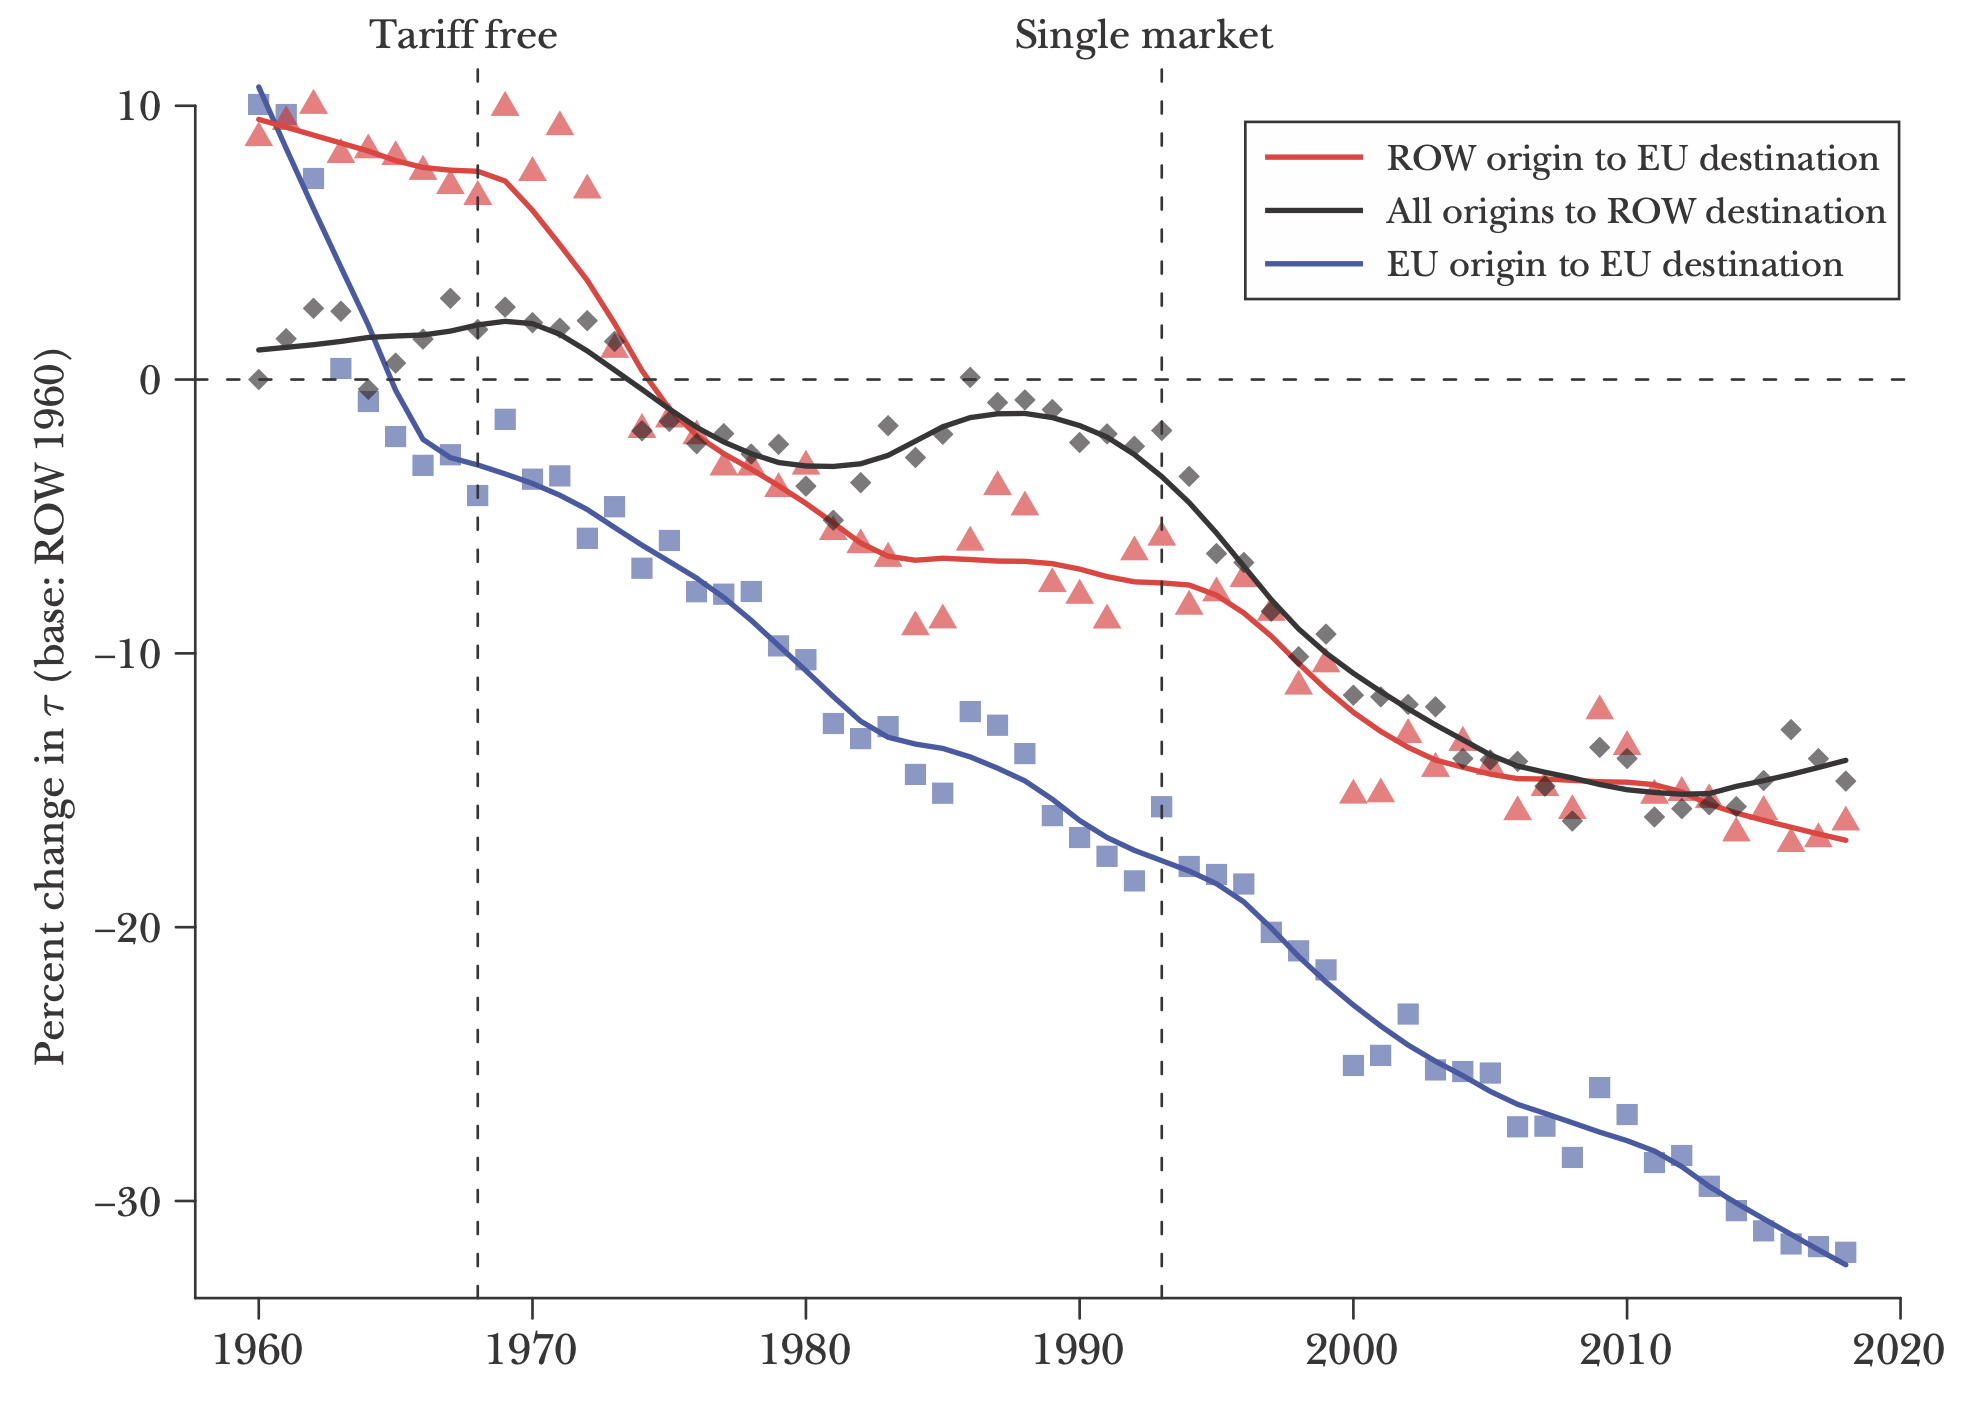
\includegraphics[width=1\textwidth]{IFME/Graphs/Europe_Trade_Costs.png}
    \label{fig:EU_Trade_Costs}
    Figure Source: \cite{US_Europe}\\ Note: \enquote{Each point is obtained by differencing with respect to the 1960 ROW-border coefficient, dividing by $- \epsilon = -5$, exponentiating, subtracting one, and multiplying by 100.} (\cite{US_Europe})
\end{figure} Figure \ref{fig:EU_Trade_Costs} presents the evolution of total trade costs between 1960 and 2018, taking 1960 as a reference year (\cite{US_Europe}). The blue line and squares indicate the change in trade costs between economies that are members of the EU. The red line and triangles illustrate the difference in trade costs compared to the base year for imports from non-EU countries into the EU. The change in trade costs for all trade flows recorded outside the EU is represented by the black line and diamonds. All differences are expressed in percent. The figure shows that in 1960, the costs related to trade to or within the EU were about 10 percent higher, compared to transactions outside the EU. In the subsequent years, a decline in trade costs compared to the base year can be observed, potentially driven in part by the abolishment of tariffs and a closer economic integration between EU member countries. \textcite{US_Europe} state that in 2018, a decrease of trade costs of about 38 percent compared to 1960 can be observed. In contrast, it can be observed that the reduction in trade costs for imports from non-EU members to the EU, as well as trade flows observed outside the EU, showed a less pronounced reduction compared to the base year. However, \textcite{US_Europe} find that trade costs still decreased by about 23 percent compared to 1960 in the case of imports to the EU from outside. 

The above findings indicate that an overall reduction of trade costs has been realised in the past sixty years, regardless of EU membership. However, the effect is more pronounced for trade between EU-countries, supporting the arguments presented in Section \ref{EPF}, that increased economic integration among countries - such as through FTAs, EU-membership, or a common currency - significantly lowers bilateral trade costs. 

































Another discipline that gravity equations can be used for is the estimation of welfare gains from trade liberalization (\cite{old_gains}). A key figure in that regard is the trade cost elasticity of trade as an indicator for the responsiveness of trade flows when costs change. \textcite[p. 163]{cookbook} identify 32 prior papers that estimate such an elasticity by (i) either using a regression framework in which bilateral trade costs (if available) and competitiveness indicators like wage costs, productivity measures or exchange rates are utilized to explain trade flows, or (ii) the elasticity is recovered from ($1-\sigma$) as in equation \ref{eq:bil_trade_costs_SGE} mentioned in section \ref{subsec:estimation_tools}. They provide summary statistics on the trade cost elasticity of trade. These can be seen in table \ref{tab:elasticities_trade_costs}.



\begin{table}[htbp]
    \centering
    \caption[Descriptive Statistics of Price Elasticities in Gravity Equations]{Descriptive Statistics of Price Elasticities in Gravity Equations}
    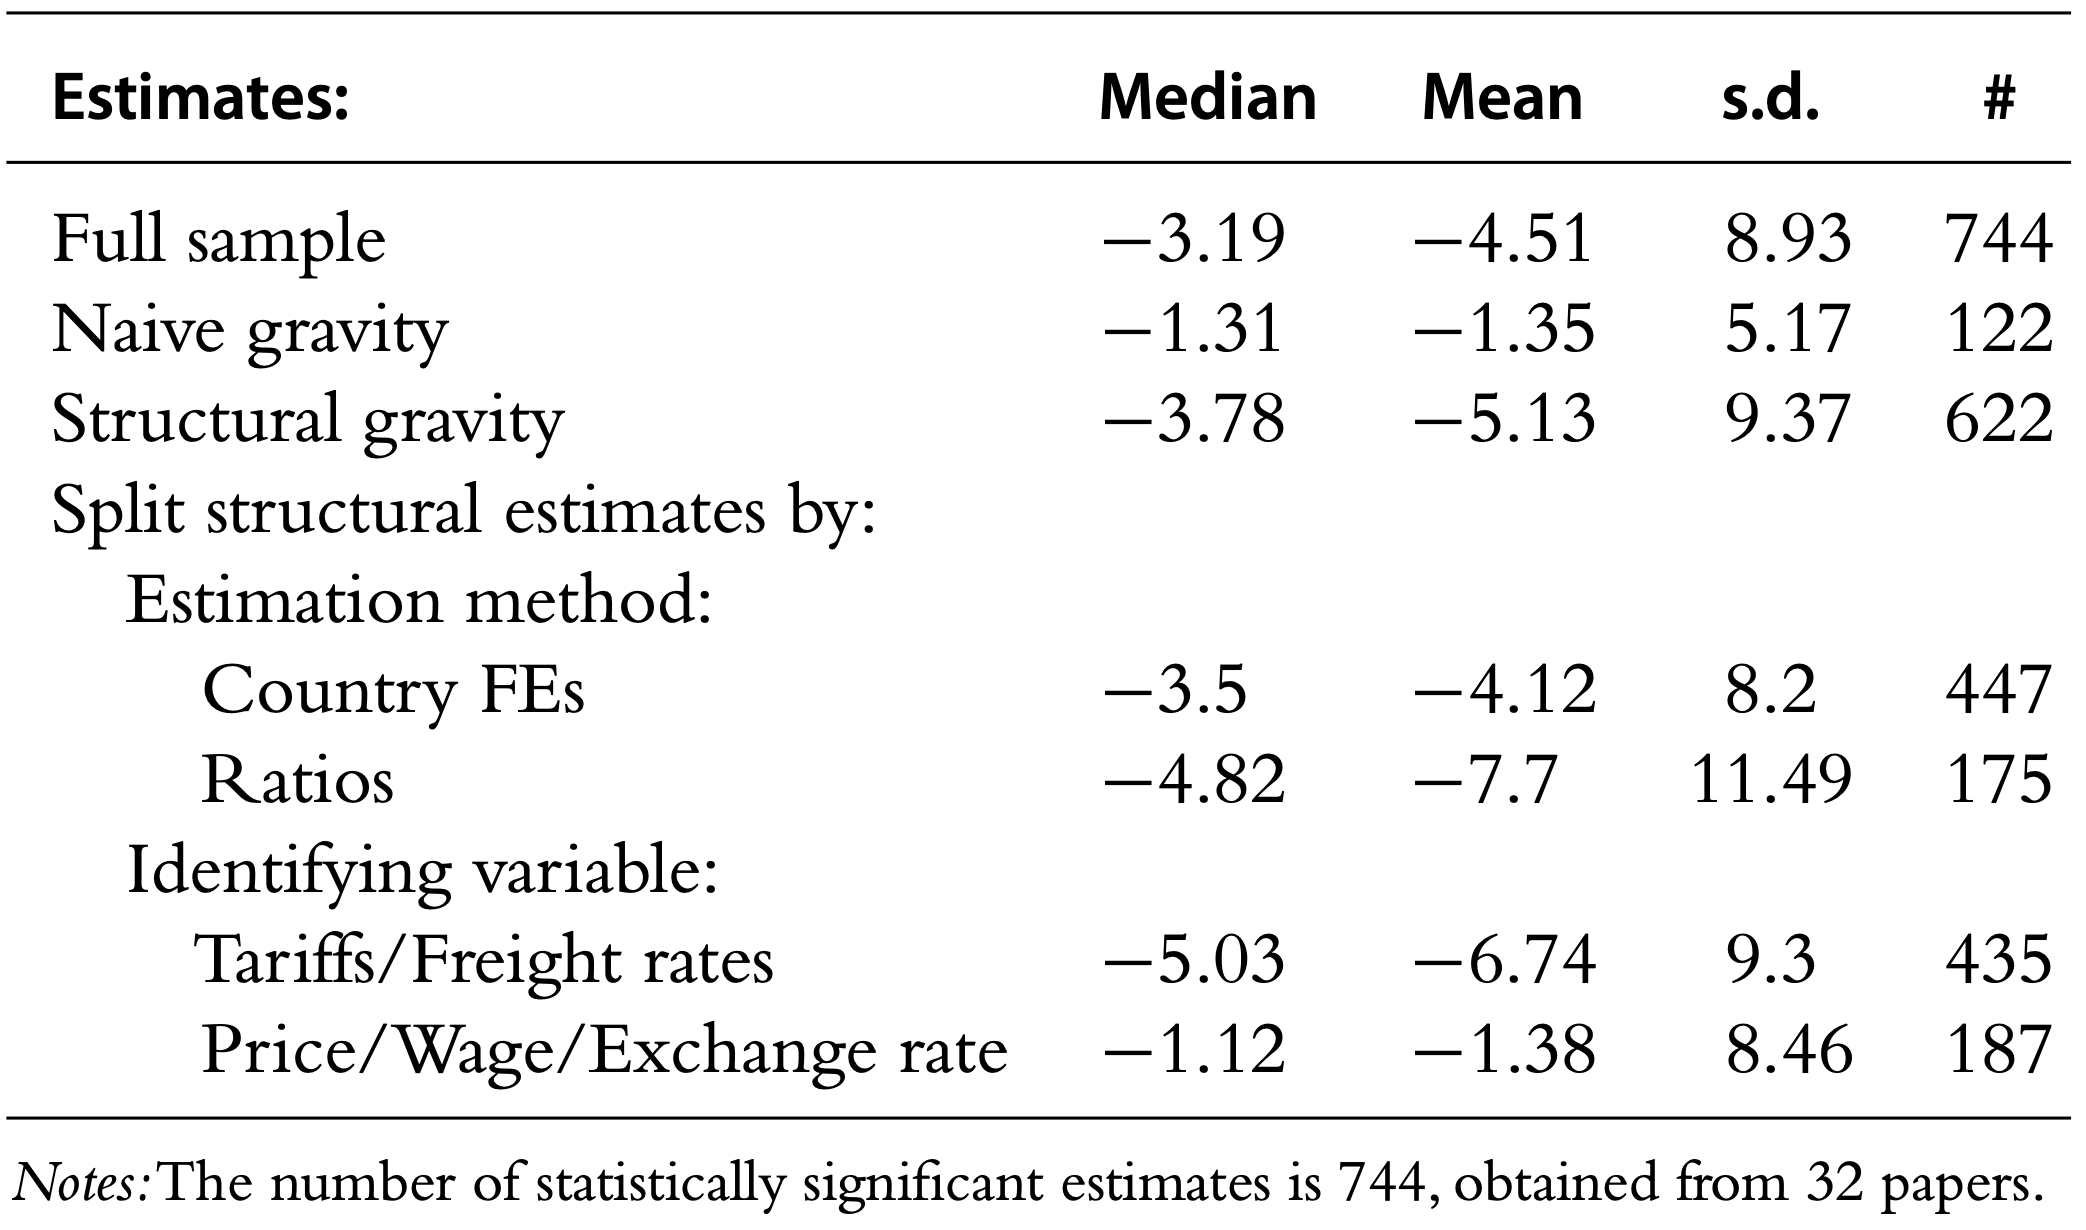
\includegraphics[width=1\textwidth]{IFME/Graphs/elasticities_of_trade_costs.png}
    \label{tab:elasticities_trade_costs}
    Table Source: \cite[p. 164]{cookbook}
\end{table}





Note that the summary statistics were split beginning from the forth row. First, \textcite[p. 164]{cookbook} divide the sample into models that include mutlilateral resistance by either fixed effects or the use of proper ratios, neglecting all studies that have made the \textit{gold medal mistake}. Secondly, only including the filtered studies above, they further split the sample by the covariates included in the regression (see the last two rows of table \ref{tab:elasticities_trade_costs}). The high standard deviation of all the estimates (especially in comparison to the mean) can be traced back to (i) heterogeneity across firms, since many of the papers estimate on the firm level and (ii) the different specifications (\cite[p. 164-165]{cookbook}). Overall, table \ref{tab:elasticities_trade_costs} shows that all mean estimates of trade elasticities with respect to trade costs are larger than one, indicating a general elastic reaction of trade to a change in trade costs. Having an accurate measure of trade elasticities with respect to trade costs is crucial for policy decisions because it determines how significantly trade flows respond to changes in trade barriers, thereby shaping the effectiveness and outcomes of trade liberalization efforts (\cite[p. 165]{cookbook}).





































\subsection[Results of Service Trade Applications]{Results of Service Trade Applications$^{\text{ JE}}$}
\label{sec:Service_Models}


This subsection aims at highlighting the special attributes when it comes to international trade in services and reviews some findings of gravity model applications that quantify effects of trade barriers on cross-border services. Since services are intangible by nature (\cite{intangible_2023}, \cite{eurostat2002manual}), a wide range of classifications into different categories and along different dimensions exists in the literature. A prominent distinction is made by defining the way, in which a service can be supplied across a border. 




\begin{figure}[htbp]
    \centering
    \caption[Synthetic view of modes of service supply]{Synthetic view of modes of service supply set by the \textcite{eurostat2002manual}}
    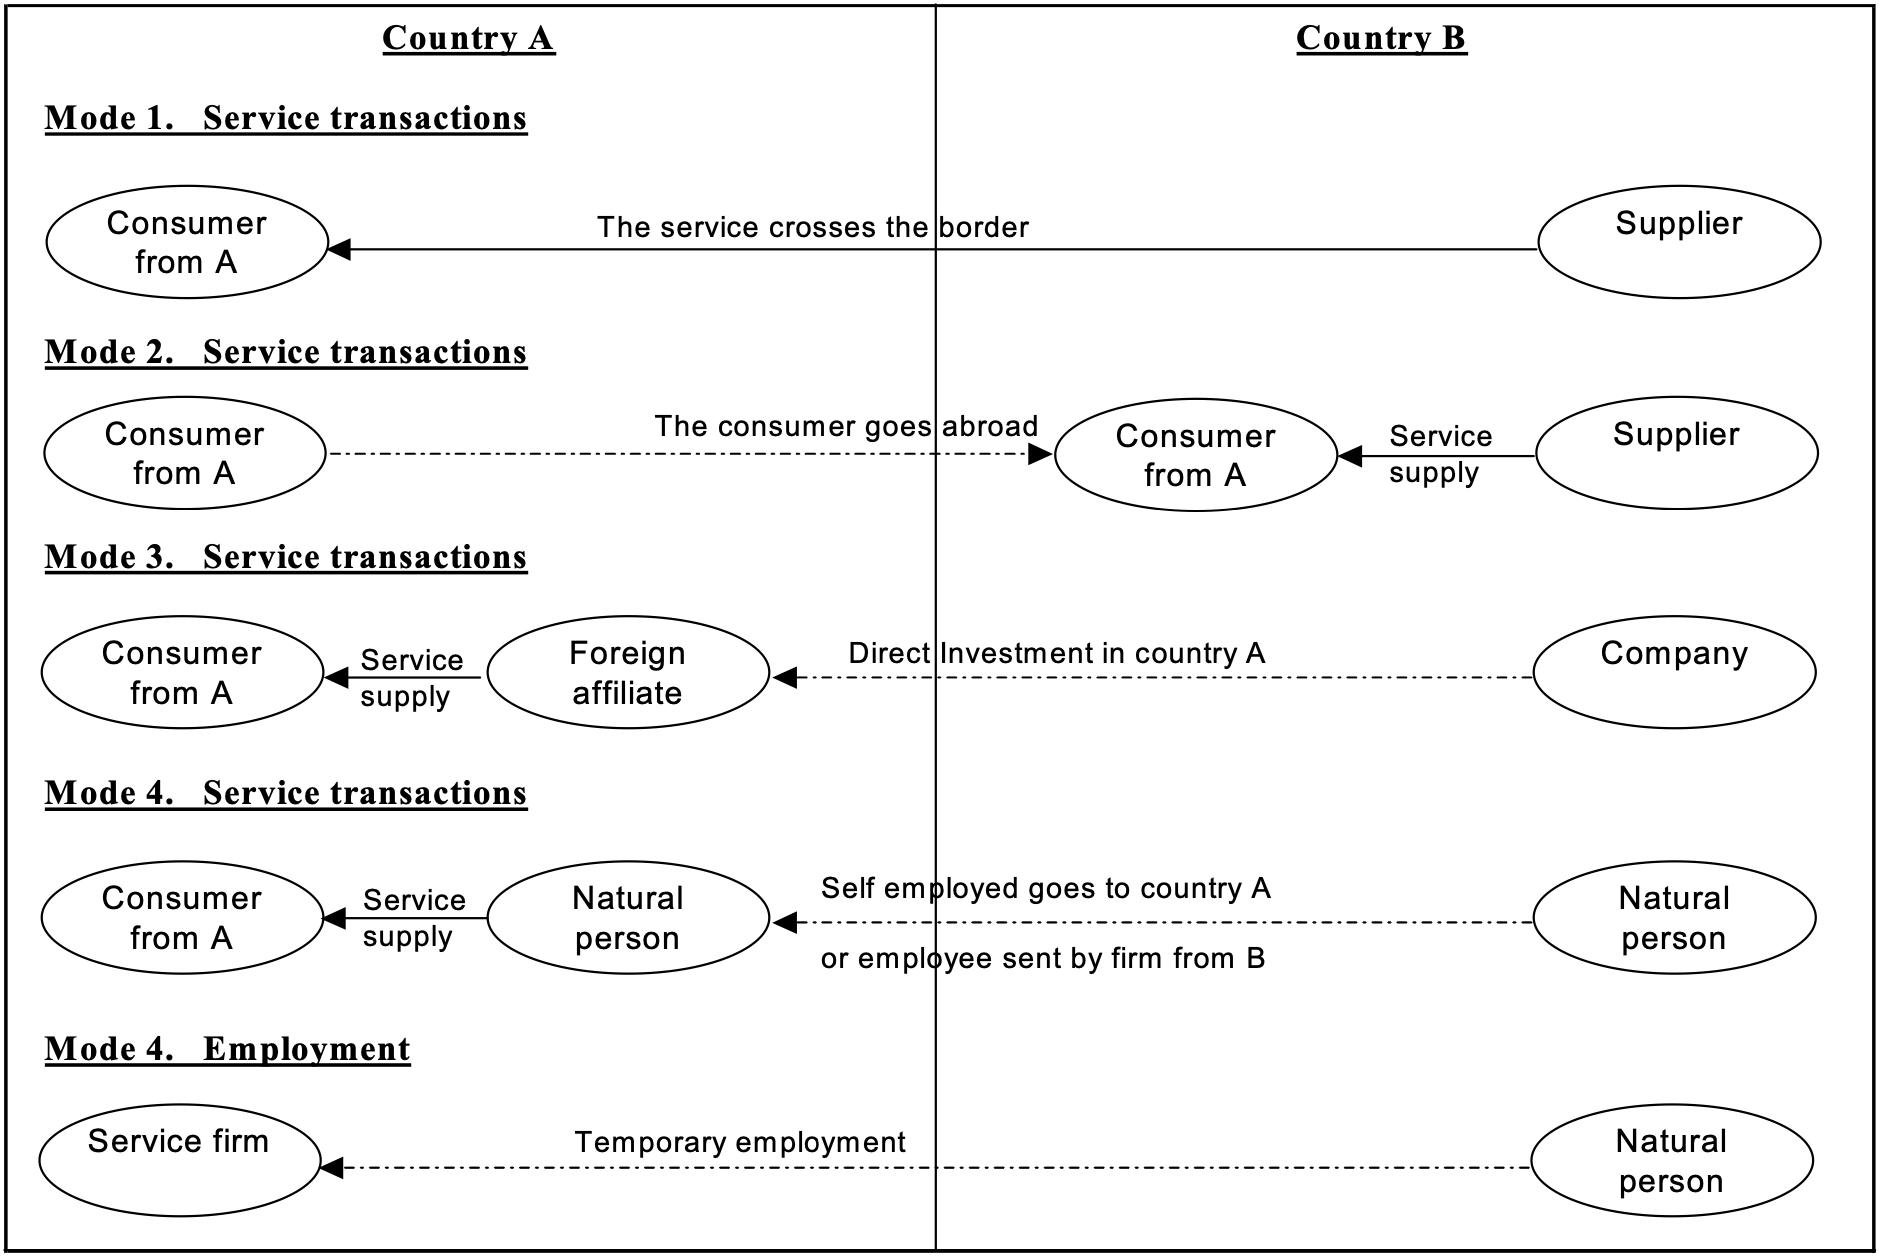
\includegraphics[width=1\textwidth]{IFME/Graphs/Service_supply_modes.png}
    \label{fig:service_modes}
    \small 
    Figure Source: \cite[p. 25]{eurostat2002manual}
\end{figure}



The four modes that supply of services trade (from here called \textit{mode x}) could take are defined in the General Agreement on Trade in Services (GATS). Broadly, \textit{mode 1} can be summarized as the cross-border supply of services, \textit{mode 2} represents service consumption abroad, \textit{mode 3} stands for the commercial presence of foreign service companies and finally, \textit{mode 4} includes all cross-border movements of natural persons. Figure \ref{fig:service_modes} illustrates these modes and provides intuition of real world applications.









\textcite{Breinlich_and} also highlight the relatively higher importance of heterogeneity across firms when it comes to trade in services compared to trade in goods. They mainly provide a classification of three important classes of services when it comes to international trade: (i) producer services (inputs in production of other services and goods), (ii) services that involve travel of persons and (iii) transportation services. Along these classes they identify differences in (i) the number of foreign markets served, (ii) the value of exports and imports per served market and (iii) the share of individual markets in overall sales. 

To present stylized facts about trade in services \textcite{Breinlich_and} assess how well heterogeneous firms gravity models from the literature can be utilized to construct analysis in service sectors. They find that a large amount of the existing covariates (language dummy, border dummy, colonial ties and so on) are also determinants for trade in services and therefore, such models are implied to be a starting point for further empirical studies.\footnote{This is inline with findings of \textcite{Walsh2006}, who also points out that the gravity equation can be used well to asses determinants of services trade, once empirical estimation tools overcome sources of bias, like firm heterogeneity.} Merging the Annual Respondents Database for the UK and the International Trade in Services Inquiry, \textcite{Breinlich_and} produce a rather disaggregated dataset to determine the extensive margin (number of traders and service types per country) and intensive margin (average trade per firm and service type) an thus, explain micro patterns of services trade. They also indirectly imply that trade barriers for services differ in their nature from barriers for goods. 




Generally, the assessment and estimation of trade barriers in services trade is more complex than in goods trade and therefore, harder to quantify in an empirical setup. Trade barriers in services trade often take the form of legal or institutional regulations, instead of tariffs or other \textit{easily} quantifiable barriers when it comes to goods trade (\cite{Trade_Barriers_Korea}). Imposing tariffs or restricting services through import quotas turns out to be difficult for a service when referring to the original definition, in which the supply and consumption of a service occurs simultaneously (\cite{Trade_Barriers_Korea}). Therefore, regulations that classify as trade barriers in services are usually laid upon the providing firms themselves. Broadly, \textcite{Trade_Barriers_Korea} summarize examples for such service trade barriers as (i) obtaining licenses (induced with cross-border restrictions), (ii) environmental regulations and standards, (iii) acceptance and refusal of certificates and academic degrees, (iv) government service demand policies that favor domestic providers and finally, (v) exporting service firms often need to utilize foreign distribution networks or existing infrastructure. Any regulation that systematically discriminates foreign service providers from using these networks compared to domestic ones can also be classified as a service trade barrier. \textcite{Trade_Barriers_Korea} continue to first estimate the structural gravity model (without the inclusion of mutlilateral resistance terms) excluding trade barriers in the model. The fitted values of that model are then used to forecast trade flows. These forecasts are than compared to actually observed data. \textcite{Trade_Barriers_Korea} use the observed differences backwards to proxy trade barriers with the focus on business, financial and transportation services due to limited data availability. Their main result is the estimation of tariff equivalents for different countries that describes in percentage (relative to a benchmark country with the lowest estimated trade barriers) how strong trade barriers in services are. 







\textcite{intangible_2023} investigate sector heterogeneity when it comes traded services and give more detailed insights into different trade barriers for different industries. They provide a rich class categories to describe different aspects in this field. First, they split the underlying characteristics among different service industries into the three dimensions (i) \textit{the level of customer interaction needed}, (ii) \textit{the level of online marketability} and \textit{the level of skill required to supply the service}. Using the modes of service supply as discussed above and shown in figure \ref{fig:service_modes}, \textcite{intangible_2023} apply the idea of these dimensions to the different industries and argue that some sectors might utilize all four modes (e.g. legal services), while others predominantly supply through one mode (e.g. travel and tourism, as this mainly involves mode 2). They continue by considering 13 different service sectors and place them into three parent categories: (i) \textit{data-intensive services}\footnote{As \textit{data-intensive services} \textcite{intangible_2023} list \enquote{telecommunications, computer, and insurance services}.}, (ii) \textit{transportation and related services}\footnote{As \textit{transportation and related services} \textcite{intangible_2023} list \enquote{air transport, road, rail, and sea freight transport, logistics, and postal and courier services}.} and (iii) \textit{professional and related services}\footnote{As \textit{professional and related services} \textcite{intangible_2023} list \enquote{legal, accounting, architecture and engineering, and construction services}.}. Furthermore, \textcite{intangible_2023} proceed by analyzing the sub-sectors of these broader categories through the decomposition of the STRI along the four modes of supply from figure \ref{fig:service_modes}.


\begin{figure}[ht]
    \centering
    \caption[Average STRI scores by mode of supply, 2014-2017.]{Average STRI scores by mode of supply, 2014-2017.}
    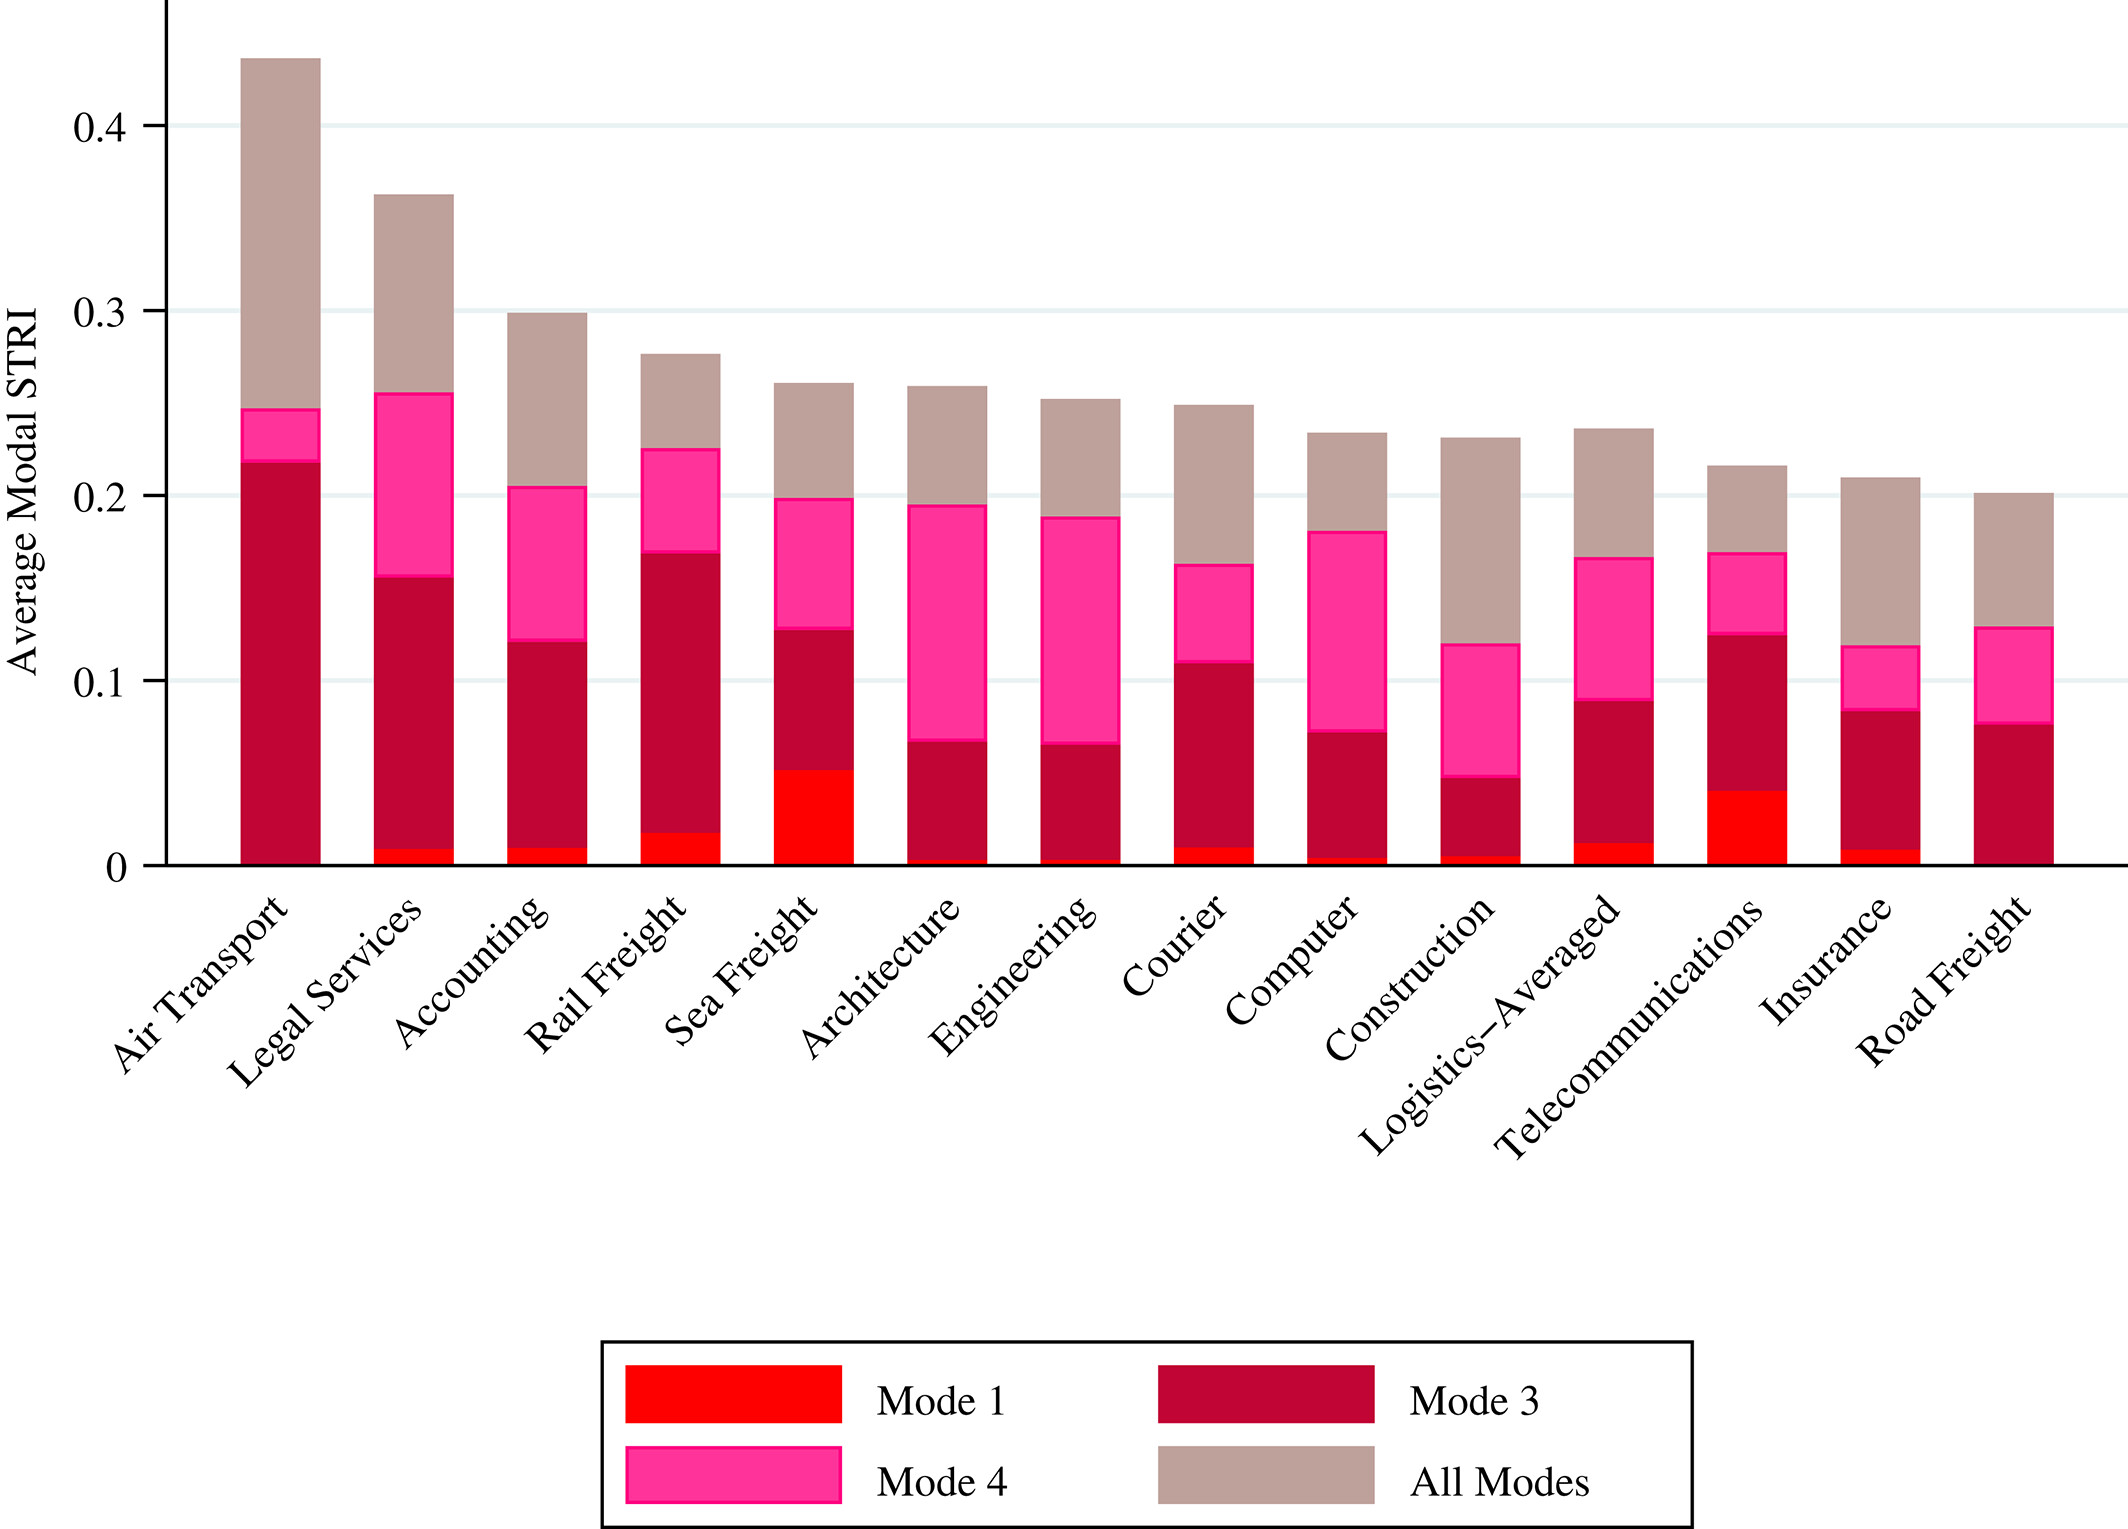
\includegraphics[width=1\textwidth]{IFME/Graphs/STRI_mode.jpeg}
    \label{fig:STRI_modes}
    \small 
    \enquote{Modal STRI values averaged over the years and observations in the data sample.} \\
    Figure Source: \cite{intangible_2023} \\ Online Link: \href{https://onlinelibrary.wiley.com/doi/10.1111/twec.13346  }{wileyonlinelibrary.com}
\end{figure}



Figure \ref{fig:STRI_modes} shows how the reviewed industries' STRI\footnote{Logistics sector is excluded.} looks disaggregated across the modes of supply. Note that mode two is not included, since mode two is characterized by the mobility of the customer (see figure \ref{fig:service_modes}). Therefore, any trade barriers that are relevant for that mode mainly depend on bilateral regulations (e.g. visa requirements) and must not be distinguished on the sector level (\cite{intangible_2023}). Mainly, figure \ref{fig:STRI_modes} provides insights which types of regulations that act as service trade barriers are important for which industries, and to what extent. For instance, computer services can be seen to be effected very little by mode one barriers like data flow restrictions, while mode four barriers - like temporary entry limits of natural persons - restrict computer services trade relatively strong. The authors find adequate words to explain this: \enquote{While many of the activities that fall under computer services, such as electronic delivery of software, do not require physical presence to export, other services, such as cloud infrastructure, tend to benefit from local infrastructure to improve customer experience.} (\cite{intangible_2023}). Figure \ref{fig:STRI_modes} also shows that air transport services are, on average, the most restricted in the selected sample, mainly by regulations that effect all supply modes and specifically mode 3 policies such as foreign equity participation or public ownership (\cite{intangible_2023}). Disaggregating these trade barriers subject to the shown industries sheds light on the often unobserved heterogeneity in services trade by sectors. Another example is the telecommunications industry, for which mode three barriers make up relatively most of the overall STRI. \textcite{intangible_2023} point out that antitrust regulations on \enquote{[…] cross-border mergers and acquisitions, foreign branch limits and data flow restrictions} can be seen as the most important ones for this sector.\footnote{To find further insights on specific policies that hamper trade in the respective industries, see \textcite{intangible_2023}.} 

The main value \textcite{intangible_2023} then add to the literature is by using the structural gravity model to investigate the relationship of mode three barriers (e.g. limitations on foreign equity shares) to traded services in all other modes. Contrary to findings before, they conclude that mode three trade acts complementary to the other modes, instead of having a substitutable nature. The intuition is as follows. If mode three trade and the rest of the modes are assumed to be substitutes, a policy that would reduce mode three trade - like restrictions on foreign direct investments (FDI) in foreign affiliates - would lead to a rise in services trade in the other modes. In that case it is implied that welfare reductions due to less trade in mode three are compensated to some extent by the achieved trade gains from the other modes. The opposite would be the case if a complementary relationship is assumed. A regulation aimed at reducing FDI would lead to less exports in mode 3 services as well as the other modes. In combination with their finding of a complementary relationship, \textcite{intangible_2023} therefore conclude that policies to liberalize mode three trade can positively effect welfare through gains from trade in all service modes.

In addition to this, \textcite{trade_agreements_2024} explore the impact of trade agreements on services trade, providing a differentiated analysis of different types of agreements, particularly General Trade Agreements (GTAs) and Deep Trade Agreements (DTAs). While tariff reductions through RTAs are found to boost trade in goods strongly, their effect on services trade is smaller (\cite{trade_agreements_2024}). Their primary contribution lies in examining the heterogeneous effects of these agreements, noting that higher institutional quality in high-income countries leads to stronger service market integration. \textcite{trade_agreements_2024} highlight the effectiveness of DTAs by addressing behind-the-border barriers, thereby lowering service trade costs and improving the business environment. They use the PPML estimator within a difference-in-differences framework to be able to also make causal conclusions.\footnote{\textcite{trade_agreements_2024} also provide robustness checks to mitigate potential endogeneity concerns and use propensity score matching to address the self-selection bias of RTAs.}









To highlight the wide range of possible applications of the gravity framework, we want to mention two more aspects that help to better understand the complex nature of services trade. First, \textcite{religion} shows that religion can also be viewed as a determinant of trade and effects international trade through two channels. The first one are network effects that can be generated by enhancing trust between trading partners that share the same religious beliefs and thus, bilateral distance in the sense of transaction costs can be reduced. Secondly, heterogeneous institutional effects take place, i.e. some religious regimes promote openness and trade, whereas others hamper it.\footnote{\textcite{religion} does also not analyse the extant of heterogeneity relating to the institutional effects of religion on trade. Their implications can only be interpreted at the aggregate level.} Overall, \textcite{religion} uses a gravity based PPML estimation approach without incorporation of multilateral resistance terms (thus, committing the gold medal mistake)\footnote{Therefore, the implications have to be considered with great care.} to find that a common religion fosters trade through these two channels. Interestingly, \textcite{religion} also run their model both on trade in goods and trade in services and show that the impact of religion is larger in services sectors than in goods sectors. This finding highlights again the nature of services trade, in which suppliers and consumers have to engage in a more close relationship than, for instance, a firm that exports merchandise to its customers.  



Finally, the above mentioned network effects and interdependencies are of special importance and become more frequently addressed in recent literature. As pointed out by \textcite{understanding_2023}, the inclusion of proper mutlilateral resistance terms reflect to some extent such network interdependencies, however, only on the surface level. In reality, global value chains become more complex and intermediate inputs in the production of goods and services are increasingly characterized by non-physical attributes (\cite{understanding_2023}). Especially digital services as intermediate inputs in global value chains develop quickly and are complex in nature. \textcite{understanding_2023} therefore utilize a social network approach, accounting for the \textit{connectivity} of trading partners with their respective trading partners' partners. They use this method to create network interdependency indicators which they then include in a two-stage gravity model approach, where the first stage is computed using the PPML estimator and the second stage, including the constructed indicators, is estimated using OLS.\footnote{\textcite{understanding_2023} carefully examine the inclusion of fixed effects as well as multilateral resistance terms in their two-stage estimation process and reflect on potential sources of bias.} Their findings indicate that the cross-border digital services embodied in gross exports build an even more heterogeneous value chain network than that of the general global trade. Moreover, \textcite{understanding_2023} point out that market access costs of firms engaged in cross-border digital services can be substantially lowered by having a strengthened network, including well connected trading partners. The intuition is that knowledge spill-overs of partner firms can ease the entrance of new foreign markets by implicitly lowering service trade barriers (\cite{understanding_2023}). As digital services rapidly evolve and technological progress might face a new era of growth due to new discoveries in the field of convolutional neuronal networks and artificial intelligence, ongoing research on the heterogeneous nature and complexity of global digital service networks will be needed to understand future trade dynamics.













\section[Conclusion]{Conclusion$^{\text{ JE, MK}}$}
\label{sec:conclusion}

In this seminar paper, we provided an overview on how the gravity framework, the related theoretical approaches and estimation have evolved. We showed that beside the \textit{usual} determinants - economic mass and distance - other factors representing trade costs and barriers, such as cultural distance and geographical features, may not be neglected while constructing a gravity model. Another main finding of this seminar paper is how the importance of different factors varies when considering at goods, on the one, and services, on the other hand. 

The increasing relevance of services in the composition of trade flows demands for an in-depth analysis of services trade as also reflected by the growing literature in this field yielding valuable information and implications to policy makers. Furthermore, combining the gravity-based approaches with other tools, such as social network analysis, gives more detailed insights to complex interdependencies and global value chains. Another conclusion is that, especially in services trade, sector and firm level heterogeneity should not be neglected and disaggregated analysis should be preferred. We predict that gravity equations will not soon disappear from the landscape of empirical literature on international trade. 
























































% \input{Contents/Section-6}

%\input{Contents/Section-7}
%\newpage
%\input{Contents/Section-8}
%\newpage
%\input{Contents/Section 9}
%\newpage
%\input{Contents/Section 10}
%\newpage





%\begin{appendix}


%\renewcommand{\thesubsection}{A\arabic{subsection}}
%\renewcommand{\thetable}{A\arabic{subsection}.\arabic{table}}
%\counterwithin{table}{subsection}
%\counterwithin{figure}{subsection}












%==============================References===========================
\newpage


\vspace*{-1cm}
% \addcontentsline{toc}{section}{References}


%\renewcommand\refname{References} % name for the reference list
%{\setstretch{1.0} % linespacing for the references
%\addcontentsline{toc}{section}{References} % to change the name of the references in the TOC
%\bibliography{References.bib} % adds the references to the document
%}




\sloppy

\pagenumbering{Roman} % starting roman page numbering
\setcounter{page}{6}


\phantomsection
\addcontentsline{toc}{section}{References}

\printbibliography[title={References},
%heading=bibintoc, 
]
\newpage

\fussy
%================================================================

% \begin{appendix}










\vspace*{-1.5cm}
% \vspace{1.5cm}
\appendix

\section*{Appendix}
\setcounter{section}{0}
 \addcontentsline{toc}{section}{Appendix}
\vspace*{0.5cm}
% \renewcommand{\thesection}{}
% \section{Additional Graphs}




% \newpage
% \vspace*{-1.5cm}
% \section{Additional Tables}










% \newpage
% \vspace*{-1.5cm}
\section{Author Index}


\vspace{2cm}








\begin{table}[h]
\centering
\caption{Author Index}
\label{tab:author_index}
\begin{tabular}{|p{3cm}|p{5cm}|}
\hline
\textbf{Author} & \textbf{Sections Written} \\
\hline
\vspace{1mm} Alp Akalin \vspace{1mm} & \vspace{1mm} \begin{itemize}
    \item Section \ref{sec:Introduction} 
    \item Section \ref{sec:Gravity_Framework}
    \item Section \ref{subsec:theoretic_foundations}
\end{itemize} \\
\hline
\vspace{1mm} Melanie Kortland \vspace{1mm} & \vspace{1mm} \begin{itemize}
    \item Section \ref{sec:Introduction} 
    \item Section \ref{sec:Determinants_of_Trade}
    \item Section \ref{sec:Proxies_Distance}
    \item Section \ref{sec:Proxies_Mass}
    \item Section \ref{EPF}
    \item Section \ref{sec:geo}
    \item Section \ref{sec:culture}
    \item Section \ref{sec:mobility}
    \item Section \ref{sec:other}
    \item Section \ref{sec:Goods_Models}
    \item Section \ref{sec:conclusion}
\end{itemize} \\
\hline
\vspace{1mm} Jannes Ehrhardt \vspace{1mm} & \vspace{1mm} \begin{itemize}
    \item Section \ref{sec:Introduction} 
    \item Section \ref{sec:Gravity_Framework}
    \item Section \ref{subsec:estimation_tools}
    \item Section \ref{sec:Empirical_evidence}
    \item Section \ref{sec:Goods_Models}
    \item Section \ref{sec:Service_Models}
    \item Section \ref{sec:conclusion}
\end{itemize} \\
\hline
\end{tabular}
\end{table}
\newpage

\section{Declaration of Self-Reliance}




We hereby affirm under oath that we have independently authored this work and have utilized no sources or aids other than those specified. Furthermore, we attest that we have adhered to the general principles of scientific research and publication as delineated in the guidelines of good scientific practice set forth by the Carl von Ossietzky University of Oldenburg. Any potential errors in this work are attributable to us as the authors.

\vspace{1cm}

  \noindent  Oldenburg, \today
    
    \vspace{1cm}



    


    \vspace*{-3cm}\hspace*{3.85cm}
\includegraphics[width=0.6\columnwidth]{Graphs/Unterschrift_Jannes_1.pdf} \\
  
    \vspace{-3.3cm}  
    
    \rule{\linewidth}{1pt}
    \vspace{-1.1cm}
    \begin{center}
        Jannes Ehrhardt \\
        \vspace{-0.2cm} 
        (5257507)
    \end{center}


% \end{appendix}

% \newpage





\end{document}